\documentclass[1p]{elsarticle_modified}
%\bibliographystyle{elsarticle-num}

%\usepackage[colorlinks]{hyperref}
%\usepackage{abbrmath_seonhwa} %\Abb, \Ascr, \Acal ,\Abf, \Afrak
\usepackage{amsfonts}
\usepackage{amssymb}
\usepackage{amsmath}
\usepackage{amsthm}
\usepackage{scalefnt}
\usepackage{amsbsy}
\usepackage{kotex}
\usepackage{caption}
\usepackage{subfig}
\usepackage{color}
\usepackage{graphicx}
\usepackage{xcolor} %% white, black, red, green, blue, cyan, magenta, yellow
\usepackage{float}
\usepackage{setspace}
\usepackage{hyperref}

\usepackage{tikz}
\usetikzlibrary{arrows}

\usepackage{multirow}
\usepackage{array} % fixed length table
\usepackage{hhline}

%%%%%%%%%%%%%%%%%%%%%
\makeatletter
\renewcommand*\env@matrix[1][\arraystretch]{%
	\edef\arraystretch{#1}%
	\hskip -\arraycolsep
	\let\@ifnextchar\new@ifnextchar
	\array{*\c@MaxMatrixCols c}}
\makeatother %https://tex.stackexchange.com/questions/14071/how-can-i-increase-the-line-spacing-in-a-matrix
%%%%%%%%%%%%%%%

\usepackage[normalem]{ulem}

\newcommand{\msout}[1]{\ifmmode\text{\sout{\ensuremath{#1}}}\else\sout{#1}\fi}
%SOURCE: \msout is \stkout macro in https://tex.stackexchange.com/questions/20609/strikeout-in-math-mode

\newcommand{\cancel}[1]{
	\ifmmode
	{\color{red}\msout{#1}}
	\else
	{\color{red}\sout{#1}}
	\fi
}

\newcommand{\add}[1]{
	{\color{blue}\uwave{#1}}
}

\newcommand{\replace}[2]{
	\ifmmode
	{\color{red}\msout{#1}}{\color{blue}\uwave{#2}}
	\else
	{\color{red}\sout{#1}}{\color{blue}\uwave{#2}}
	\fi
}

\newcommand{\Sol}{\mathcal{S}} %segment
\newcommand{\D}{D} %diagram
\newcommand{\A}{\mathcal{A}} %arc


%%%%%%%%%%%%%%%%%%%%%%%%%%%%%5 test

\def\sl{\operatorname{\textup{SL}}(2,\Cbb)}
\def\psl{\operatorname{\textup{PSL}}(2,\Cbb)}
\def\quan{\mkern 1mu \triangleright \mkern 1mu}

\theoremstyle{definition}
\newtheorem{thm}{Theorem}[section]
\newtheorem{prop}[thm]{Proposition}
\newtheorem{lem}[thm]{Lemma}
\newtheorem{ques}[thm]{Question}
\newtheorem{cor}[thm]{Corollary}
\newtheorem{defn}[thm]{Definition}
\newtheorem{exam}[thm]{Example}
\newtheorem{rmk}[thm]{Remark}
\newtheorem{alg}[thm]{Algorithm}

\newcommand{\I}{\sqrt{-1}}
\begin{document}

%\begin{frontmatter}
%
%\title{Boundary parabolic representations of knots up to 8 crossings}
%
%%% Group authors per affiliation:
%\author{Yunhi Cho} 
%\address{Department of Mathematics, University of Seoul, Seoul, Korea}
%\ead{yhcho@uos.ac.kr}
%
%
%\author{Seonhwa Kim} %\fnref{s_kim}}
%\address{Center for Geometry and Physics, Institute for Basic Science, Pohang, 37673, Korea}
%\ead{ryeona17@ibs.re.kr}
%
%\author{Hyuk Kim}
%\address{Department of Mathematical Sciences, Seoul National University, Seoul 08826, Korea}
%\ead{hyukkim@snu.ac.kr}
%
%\author{Seokbeom Yoon}
%\address{Department of Mathematical Sciences, Seoul National University, Seoul, 08826,  Korea}
%\ead{sbyoon15@snu.ac.kr}
%
%\begin{abstract}
%We find all boundary parabolic representation of knots up to 8 crossings.
%
%\end{abstract}
%\begin{keyword}
%    \MSC[2010] 57M25 
%\end{keyword}
%
%\end{frontmatter}

%\linenumbers
%\tableofcontents
%
\newcommand\colored[1]{\textcolor{white}{\rule[-0.35ex]{0.8em}{1.4ex}}\kern-0.8em\color{red} #1}%
%\newcommand\colored[1]{\textcolor{white}{ #1}\kern-2.17ex	\textcolor{white}{ #1}\kern-1.81ex	\textcolor{white}{ #1}\kern-2.15ex\color{red}#1	}

{\Large $\underline{12a_{0265}~(K12a_{0265})}$}

\setlength{\tabcolsep}{10pt}
\renewcommand{\arraystretch}{1.6}
\vspace{1cm}\begin{tabular}{m{100pt}>{\centering\arraybackslash}m{274pt}}
\multirow{5}{120pt}{
	\centering
	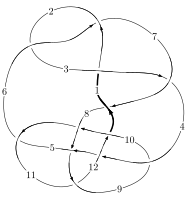
\includegraphics[width=112pt]{../../../GIT/diagram.site/Diagrams/png/1066_12a_0265.png}\\
\ \ \ A knot diagram\footnotemark}&
\allowdisplaybreaks
\textbf{Linearized knot diagam} \\
\cline{2-2}
 &
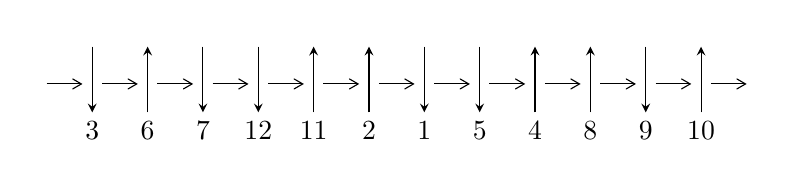
\begin{tikzpicture}[x=20pt, y=17pt]
	% nodes
	\node (C0) at (0, 0) {};
	\node (C1) at (1, 0) {};
	\node (C1U) at (1, +1) {};
	\node (C1D) at (1, -1) {3};

	\node (C2) at (2, 0) {};
	\node (C2U) at (2, +1) {};
	\node (C2D) at (2, -1) {6};

	\node (C3) at (3, 0) {};
	\node (C3U) at (3, +1) {};
	\node (C3D) at (3, -1) {7};

	\node (C4) at (4, 0) {};
	\node (C4U) at (4, +1) {};
	\node (C4D) at (4, -1) {12};

	\node (C5) at (5, 0) {};
	\node (C5U) at (5, +1) {};
	\node (C5D) at (5, -1) {11};

	\node (C6) at (6, 0) {};
	\node (C6U) at (6, +1) {};
	\node (C6D) at (6, -1) {2};

	\node (C7) at (7, 0) {};
	\node (C7U) at (7, +1) {};
	\node (C7D) at (7, -1) {1};

	\node (C8) at (8, 0) {};
	\node (C8U) at (8, +1) {};
	\node (C8D) at (8, -1) {5};

	\node (C9) at (9, 0) {};
	\node (C9U) at (9, +1) {};
	\node (C9D) at (9, -1) {4};

	\node (C10) at (10, 0) {};
	\node (C10U) at (10, +1) {};
	\node (C10D) at (10, -1) {8};

	\node (C11) at (11, 0) {};
	\node (C11U) at (11, +1) {};
	\node (C11D) at (11, -1) {9};

	\node (C12) at (12, 0) {};
	\node (C12U) at (12, +1) {};
	\node (C12D) at (12, -1) {10};
	\node (C13) at (13, 0) {};

	% arrows
	\draw[->,>={angle 60}]
	(C0) edge (C1) (C1) edge (C2) (C2) edge (C3) (C3) edge (C4) (C4) edge (C5) (C5) edge (C6) (C6) edge (C7) (C7) edge (C8) (C8) edge (C9) (C9) edge (C10) (C10) edge (C11) (C11) edge (C12) (C12) edge (C13) ;	\draw[->,>=stealth]
	(C1U) edge (C1D) (C2D) edge (C2U) (C3U) edge (C3D) (C4U) edge (C4D) (C5D) edge (C5U) (C6D) edge (C6U) (C7U) edge (C7D) (C8U) edge (C8D) (C9D) edge (C9U) (C10D) edge (C10U) (C11U) edge (C11D) (C12D) edge (C12U) ;
	\end{tikzpicture} \\
\hhline{~~} \\& 
\textbf{Solving Sequence} \\ \cline{2-2} 
 &
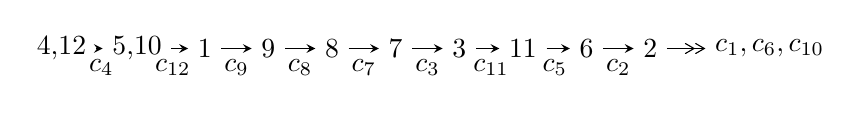
\begin{tikzpicture}[x=23pt, y=7pt]
	% node
	\node (A0) at (-1/8, 0) {4,12};
	\node (A1) at (17/16, 0) {5,10};
	\node (A2) at (17/8, 0) {1};
	\node (A3) at (25/8, 0) {9};
	\node (A4) at (33/8, 0) {8};
	\node (A5) at (41/8, 0) {7};
	\node (A6) at (49/8, 0) {3};
	\node (A7) at (57/8, 0) {11};
	\node (A8) at (65/8, 0) {6};
	\node (A9) at (73/8, 0) {2};
	\node (C1) at (1/2, -1) {$c_{4}$};
	\node (C2) at (13/8, -1) {$c_{12}$};
	\node (C3) at (21/8, -1) {$c_{9}$};
	\node (C4) at (29/8, -1) {$c_{8}$};
	\node (C5) at (37/8, -1) {$c_{7}$};
	\node (C6) at (45/8, -1) {$c_{3}$};
	\node (C7) at (53/8, -1) {$c_{11}$};
	\node (C8) at (61/8, -1) {$c_{5}$};
	\node (C9) at (69/8, -1) {$c_{2}$};
	\node (A10) at (11, 0) {$c_{1},c_{6},c_{10}$};

	% edge
	\draw[->,>=stealth]	
	(A0) edge (A1) (A1) edge (A2) (A2) edge (A3) (A3) edge (A4) (A4) edge (A5) (A5) edge (A6) (A6) edge (A7) (A7) edge (A8) (A8) edge (A9) ;
	\draw[->>,>={angle 60}]	
	(A9) edge (A10);
\end{tikzpicture} \\ 

\end{tabular} \\

\footnotetext{
The image of knot diagram is generated by the software ``\textbf{Draw programme}" developed by Andrew Bartholomew(\url{http://www.layer8.co.uk/maths/draw/index.htm\#Running-draw}), where we modified some parts for our purpose(\url{https://github.com/CATsTAILs/LinksPainter}).
}\phantom \\ \newline 
\centering \textbf{Ideals for irreducible components\footnotemark of $X_{\text{par}}$} 
 
\begin{align*}
I^u_{1}&=\langle 
1.30744\times10^{71} u^{76}+3.22892\times10^{71} u^{75}+\cdots+3.31124\times10^{66} b+7.87073\times10^{71},\\
\phantom{I^u_{1}}&\phantom{= \langle  }-2.93126\times10^{71} u^{76}-5.90588\times10^{71} u^{75}+\cdots+1.65562\times10^{66} a-1.20168\times10^{72},\;u^{77}+u^{76}+\cdots+2 u+1\rangle \\
I^u_{2}&=\langle 
-6.34090\times10^{421} u^{101}-2.36894\times10^{422} u^{100}+\cdots+1.13936\times10^{422} b-4.46492\times10^{422},\\
\phantom{I^u_{2}}&\phantom{= \langle  }5.97619\times10^{421} u^{101}+2.38844\times10^{422} u^{100}+\cdots+1.13936\times10^{422} a+8.88412\times10^{422},\\
\phantom{I^u_{2}}&\phantom{= \langle  }u^{102}+4 u^{101}+\cdots+15 u+2\rangle \\
I^u_{3}&=\langle 
- u^{26}+u^{25}+\cdots+b+4 u,\;-4 u^{26}+4 u^{25}+\cdots+a-1,\;u^{27}- u^{26}+\cdots-4 u^2+1\rangle \\
I^u_{4}&=\langle 
- u^3- u^2+b-3 u-1,\;- u^3- u^2+a-3 u-1,\;u^4+u^3+3 u^2+u+1\rangle \\
\\
\end{align*}
\raggedright * 4 irreducible components of $\dim_{\mathbb{C}}=0$, with total 210 representations.\\
\footnotetext{All coefficients of polynomials are rational numbers. But the coefficients are sometimes approximated in decimal forms when there is not enough margin.}
\newpage
\renewcommand{\arraystretch}{1}
\centering \section*{I. $I^u_{1}= \langle 1.31\times10^{71} u^{76}+3.23\times10^{71} u^{75}+\cdots+3.31\times10^{66} b+7.87\times10^{71},\;-2.93\times10^{71} u^{76}-5.91\times10^{71} u^{75}+\cdots+1.66\times10^{66} a-1.20\times10^{72},\;u^{77}+u^{76}+\cdots+2 u+1 \rangle$}
\flushleft \textbf{(i) Arc colorings}\\
\begin{tabular}{m{7pt} m{180pt} m{7pt} m{180pt} }
\flushright $a_{4}=$&$\begin{pmatrix}1\\0\end{pmatrix}$ \\
\flushright $a_{12}=$&$\begin{pmatrix}0\\u\end{pmatrix}$ \\
\flushright $a_{5}=$&$\begin{pmatrix}1\\u^2\end{pmatrix}$ \\
\flushright $a_{10}=$&$\begin{pmatrix}177049. u^{76}+356717. u^{75}+\cdots+2.31166\times10^{6} u+725817.\\-39484.9 u^{76}-97513.7 u^{75}+\cdots-691926. u-237697.\end{pmatrix}$ \\
\flushright $a_{1}=$&$\begin{pmatrix}213753. u^{76}+298403. u^{75}+\cdots+1.52213\times10^{6} u+328591.\\-109347. u^{76}-197571. u^{75}+\cdots-1.20523\times10^{6} u-352541.\end{pmatrix}$ \\
\flushright $a_{9}=$&$\begin{pmatrix}216534. u^{76}+454230. u^{75}+\cdots+3.00359\times10^{6} u+963514.\\-39484.9 u^{76}-97513.7 u^{75}+\cdots-691926. u-237697.\end{pmatrix}$ \\
\flushright $a_{8}=$&$\begin{pmatrix}216534. u^{76}+454230. u^{75}+\cdots+3.00359\times10^{6} u+963514.\\-39484.9 u^{76}-97513.7 u^{75}+\cdots-691926. u-237697.\end{pmatrix}$ \\
\flushright $a_{7}=$&$\begin{pmatrix}174969. u^{76}+449646. u^{75}+\cdots+3.26129\times10^{6} u+1.11170\times10^{6}\\199191. u^{76}+247170. u^{75}+\cdots+1.13303\times10^{6} u+186587.\end{pmatrix}$ \\
\flushright $a_{3}=$&$\begin{pmatrix}-228577. u^{76}-539101. u^{75}+\cdots-3.65918\times10^{6} u-1.25213\times10^{6}\\-289691. u^{76}+11209.4 u^{75}+\cdots+1.42905\times10^{6} u+1.31972\times10^{6}\end{pmatrix}$ \\
\flushright $a_{11}=$&$\begin{pmatrix}466449. u^{76}+774901. u^{75}+\cdots+4.50264\times10^{6} u+1.22728\times10^{6}\\-143349. u^{76}-278927. u^{75}+\cdots-1.77528\times10^{6} u-546149.\end{pmatrix}$ \\
\flushright $a_{6}=$&$\begin{pmatrix}-508259. u^{76}-260806. u^{75}+\cdots+67914.3 u+1.04200\times10^{6}\\322346. u^{76}+230196. u^{75}+\cdots+431531. u-430287.\end{pmatrix}$ \\
\flushright $a_{2}=$&$\begin{pmatrix}-2.09543\times10^{6} u^{76}-2.05278\times10^{6} u^{75}+\cdots-8.27941\times10^{6} u+429977.\\728151. u^{76}+1.13395\times10^{6} u^{75}+\cdots+6.79368\times10^{6} u+1.68063\times10^{6}\end{pmatrix}$\\&\end{tabular}
\flushleft \textbf{(ii) Obstruction class $= -1$}\\~\\
\flushleft \textbf{(iii) Cusp Shapes $= 928131. u^{76}-1.10298\times10^{6} u^{75}+\cdots-1.45398\times10^{7} u-8.87559\times10^{6}$}\\~\\
\newpage\renewcommand{\arraystretch}{1}
\flushleft \textbf{(iv) u-Polynomials at the component}\newline \\
\begin{tabular}{m{50pt}|m{274pt}}
Crossings & \hspace{64pt}u-Polynomials at each crossing \\
\hline $$\begin{aligned}c_{1}\end{aligned}$$&$\begin{aligned}
&u^{77}+37 u^{76}+\cdots-7 u-16
\end{aligned}$\\
\hline $$\begin{aligned}c_{2},c_{6}\end{aligned}$$&$\begin{aligned}
&u^{77}-5 u^{76}+\cdots-33 u+4
\end{aligned}$\\
\hline $$\begin{aligned}c_{3}\end{aligned}$$&$\begin{aligned}
&u^{77}+5 u^{76}+\cdots+17874 u+1768
\end{aligned}$\\
\hline $$\begin{aligned}c_{4},c_{8}\end{aligned}$$&$\begin{aligned}
&u^{77}+u^{76}+\cdots+2 u+1
\end{aligned}$\\
\hline $$\begin{aligned}c_{5},c_{9}\end{aligned}$$&$\begin{aligned}
&u^{77}+3 u^{75}+\cdots-9 u+2
\end{aligned}$\\
\hline $$\begin{aligned}c_{7}\end{aligned}$$&$\begin{aligned}
&u^{77}-25 u^{76}+\cdots-818285 u+37300
\end{aligned}$\\
\hline $$\begin{aligned}c_{10},c_{12}\end{aligned}$$&$\begin{aligned}
&u^{77}-12 u^{76}+\cdots+17 u+1
\end{aligned}$\\
\hline $$\begin{aligned}c_{11}\end{aligned}$$&$\begin{aligned}
&u^{77}-42 u^{76}+\cdots+11 u-2
\end{aligned}$\\
\hline
\end{tabular}\\~\\
\newpage\renewcommand{\arraystretch}{1}
\flushleft \textbf{(v) Riley Polynomials at the component}\newline \\
\begin{tabular}{m{50pt}|m{274pt}}
Crossings & \hspace{64pt}Riley Polynomials at each crossing \\
\hline $$\begin{aligned}c_{1}\end{aligned}$$&$\begin{aligned}
&y^{77}+9 y^{76}+\cdots+401 y-256
\end{aligned}$\\
\hline $$\begin{aligned}c_{2},c_{6}\end{aligned}$$&$\begin{aligned}
&y^{77}+37 y^{76}+\cdots-7 y-16
\end{aligned}$\\
\hline $$\begin{aligned}c_{3}\end{aligned}$$&$\begin{aligned}
&y^{77}-19 y^{76}+\cdots+74410324 y-3125824
\end{aligned}$\\
\hline $$\begin{aligned}c_{4},c_{8}\end{aligned}$$&$\begin{aligned}
&y^{77}+33 y^{76}+\cdots-86 y-1
\end{aligned}$\\
\hline $$\begin{aligned}c_{5},c_{9}\end{aligned}$$&$\begin{aligned}
&y^{77}+6 y^{76}+\cdots+145 y-4
\end{aligned}$\\
\hline $$\begin{aligned}c_{7}\end{aligned}$$&$\begin{aligned}
&y^{77}+17 y^{76}+\cdots-27321142975 y-1391290000
\end{aligned}$\\
\hline $$\begin{aligned}c_{10},c_{12}\end{aligned}$$&$\begin{aligned}
&y^{77}-50 y^{76}+\cdots+83 y-1
\end{aligned}$\\
\hline $$\begin{aligned}c_{11}\end{aligned}$$&$\begin{aligned}
&y^{77}+60 y^{75}+\cdots-39 y-4
\end{aligned}$\\
\hline
\end{tabular}\\~\\
\newpage\flushleft \textbf{(vi) Complex Volumes and Cusp Shapes}
$$\begin{array}{c|c|c}  
\text{Solutions to }I^u_{1}& \I (\text{vol} + \sqrt{-1}CS) & \text{Cusp shape}\\
 \hline 
\begin{aligned}
u &= \phantom{-}0.267790 + 0.992695 I \\
a &= -0.431267 + 1.100390 I \\
b &= -0.420752 - 0.212748 I\end{aligned}
 & \phantom{-}3.46656 + 2.98634 I & \phantom{-0.000000 } 0 \\ \hline\begin{aligned}
u &= \phantom{-}0.267790 - 0.992695 I \\
a &= -0.431267 - 1.100390 I \\
b &= -0.420752 + 0.212748 I\end{aligned}
 & \phantom{-}3.46656 - 2.98634 I & \phantom{-0.000000 } 0 \\ \hline\begin{aligned}
u &= \phantom{-}0.237290 + 0.931626 I \\
a &= \phantom{-}0.199446 + 0.750390 I \\
b &= \phantom{-}0.577247 + 0.825765 I\end{aligned}
 & -0.063419 + 0.815170 I & \phantom{-0.000000 } 0 \\ \hline\begin{aligned}
u &= \phantom{-}0.237290 - 0.931626 I \\
a &= \phantom{-}0.199446 - 0.750390 I \\
b &= \phantom{-}0.577247 - 0.825765 I\end{aligned}
 & -0.063419 - 0.815170 I & \phantom{-0.000000 } 0 \\ \hline\begin{aligned}
u &= -0.300216 + 1.022690 I \\
a &= \phantom{-}0.507425 + 1.023370 I \\
b &= \phantom{-}0.414276 - 0.285176 I\end{aligned}
 & \phantom{-}1.11208 - 7.98543 I & \phantom{-0.000000 } 0 \\ \hline\begin{aligned}
u &= -0.300216 - 1.022690 I \\
a &= \phantom{-}0.507425 - 1.023370 I \\
b &= \phantom{-}0.414276 + 0.285176 I\end{aligned}
 & \phantom{-}1.11208 + 7.98543 I & \phantom{-0.000000 } 0 \\ \hline\begin{aligned}
u &= -0.188410 + 1.058390 I \\
a &= \phantom{-}0.270943 + 0.956122 I \\
b &= \phantom{-}0.259606 - 0.198061 I\end{aligned}
 & -0.984111 - 0.167610 I & \phantom{-0.000000 } 0 \\ \hline\begin{aligned}
u &= -0.188410 - 1.058390 I \\
a &= \phantom{-}0.270943 - 0.956122 I \\
b &= \phantom{-}0.259606 + 0.198061 I\end{aligned}
 & -0.984111 + 0.167610 I & \phantom{-0.000000 } 0 \\ \hline\begin{aligned}
u &= \phantom{-}0.242342 + 0.878864 I \\
a &= -0.29452 + 1.39873 I \\
b &= -0.551628 - 0.034407 I\end{aligned}
 & \phantom{-}4.85147 + 0.97941 I & \phantom{-0.000000 } 0 \\ \hline\begin{aligned}
u &= \phantom{-}0.242342 - 0.878864 I \\
a &= -0.29452 - 1.39873 I \\
b &= -0.551628 + 0.034407 I\end{aligned}
 & \phantom{-}4.85147 - 0.97941 I & \phantom{-0.000000 } 0\\
 \hline 
 \end{array}$$\newpage$$\begin{array}{c|c|c}  
\text{Solutions to }I^u_{1}& \I (\text{vol} + \sqrt{-1}CS) & \text{Cusp shape}\\
 \hline 
\begin{aligned}
u &= -0.199438 + 1.083720 I \\
a &= -0.317566 + 0.995974 I \\
b &= -0.580208 + 1.187420 I\end{aligned}
 & \phantom{-}3.66736 + 0.81055 I & \phantom{-0.000000 } 0 \\ \hline\begin{aligned}
u &= -0.199438 - 1.083720 I \\
a &= -0.317566 - 0.995974 I \\
b &= -0.580208 - 1.187420 I\end{aligned}
 & \phantom{-}3.66736 - 0.81055 I & \phantom{-0.000000 } 0 \\ \hline\begin{aligned}
u &= \phantom{-}0.239909 + 1.079520 I \\
a &= \phantom{-}0.376611 + 0.943149 I \\
b &= \phantom{-}0.681597 + 1.143600 I\end{aligned}
 & \phantom{-}1.84653 - 5.56859 I & \phantom{-0.000000 } 0 \\ \hline\begin{aligned}
u &= \phantom{-}0.239909 - 1.079520 I \\
a &= \phantom{-}0.376611 - 0.943149 I \\
b &= \phantom{-}0.681597 - 1.143600 I\end{aligned}
 & \phantom{-}1.84653 + 5.56859 I & \phantom{-0.000000 } 0 \\ \hline\begin{aligned}
u &= \phantom{-}0.055475 + 1.130470 I \\
a &= \phantom{-}0.102708 + 1.179470 I \\
b &= \phantom{-}0.177608 + 1.391890 I\end{aligned}
 & -0.297314 - 0.869794 I & \phantom{-0.000000 } 0 \\ \hline\begin{aligned}
u &= \phantom{-}0.055475 - 1.130470 I \\
a &= \phantom{-}0.102708 - 1.179470 I \\
b &= \phantom{-}0.177608 - 1.391890 I\end{aligned}
 & -0.297314 + 0.869794 I & \phantom{-0.000000 } 0 \\ \hline\begin{aligned}
u &= -0.136518 + 1.129770 I \\
a &= -0.252093 + 1.133130 I \\
b &= -0.43003 + 1.35913 I\end{aligned}
 & \phantom{-}3.55022 - 1.05637 I & \phantom{-0.000000 } 0 \\ \hline\begin{aligned}
u &= -0.136518 - 1.129770 I \\
a &= -0.252093 - 1.133130 I \\
b &= -0.43003 - 1.35913 I\end{aligned}
 & \phantom{-}3.55022 + 1.05637 I & \phantom{-0.000000 } 0 \\ \hline\begin{aligned}
u &= -0.244151 + 0.819410 I \\
a &= \phantom{-}0.20371 + 1.60022 I \\
b &= \phantom{-}0.649592 + 0.048331 I\end{aligned}
 & \phantom{-}3.79661 + 3.71278 I & \phantom{-0.000000 } 0 \\ \hline\begin{aligned}
u &= -0.244151 - 0.819410 I \\
a &= \phantom{-}0.20371 - 1.60022 I \\
b &= \phantom{-}0.649592 - 0.048331 I\end{aligned}
 & \phantom{-}3.79661 - 3.71278 I & \phantom{-0.000000 } 0\\
 \hline 
 \end{array}$$\newpage$$\begin{array}{c|c|c}  
\text{Solutions to }I^u_{1}& \I (\text{vol} + \sqrt{-1}CS) & \text{Cusp shape}\\
 \hline 
\begin{aligned}
u &= \phantom{-}0.123768 + 1.156590 I \\
a &= \phantom{-}0.247722 + 1.193980 I \\
b &= \phantom{-}0.40510 + 1.44972 I\end{aligned}
 & \phantom{-}1.61740 + 5.84088 I & \phantom{-0.000000 } 0 \\ \hline\begin{aligned}
u &= \phantom{-}0.123768 - 1.156590 I \\
a &= \phantom{-}0.247722 - 1.193980 I \\
b &= \phantom{-}0.40510 - 1.44972 I\end{aligned}
 & \phantom{-}1.61740 - 5.84088 I & \phantom{-0.000000 } 0 \\ \hline\begin{aligned}
u &= -0.471665 + 0.554278 I \\
a &= -0.100726 + 0.197032 I \\
b &= -0.574410 + 0.316752 I\end{aligned}
 & -0.31083 + 1.94641 I & \phantom{-0.000000 } 0 \\ \hline\begin{aligned}
u &= -0.471665 - 0.554278 I \\
a &= -0.100726 - 0.197032 I \\
b &= -0.574410 - 0.316752 I\end{aligned}
 & -0.31083 - 1.94641 I & \phantom{-0.000000 } 0 \\ \hline\begin{aligned}
u &= -0.240699 + 0.670164 I \\
a &= -0.38161 + 2.29089 I \\
b &= \phantom{-}0.900486 + 0.308186 I\end{aligned}
 & \phantom{-}4.01950 - 0.35456 I & \phantom{-0.000000 } 0 \\ \hline\begin{aligned}
u &= -0.240699 - 0.670164 I \\
a &= -0.38161 - 2.29089 I \\
b &= \phantom{-}0.900486 - 0.308186 I\end{aligned}
 & \phantom{-}4.01950 + 0.35456 I & \phantom{-0.000000 } 0 \\ \hline\begin{aligned}
u &= \phantom{-}0.234998 + 0.645618 I \\
a &= \phantom{-}0.58520 + 2.40806 I \\
b &= -0.932639 + 0.368794 I\end{aligned}
 & \phantom{-}5.19817 - 4.45515 I & \phantom{-0.000000 } 0 \\ \hline\begin{aligned}
u &= \phantom{-}0.234998 - 0.645618 I \\
a &= \phantom{-}0.58520 - 2.40806 I \\
b &= -0.932639 - 0.368794 I\end{aligned}
 & \phantom{-}5.19817 + 4.45515 I & \phantom{-0.000000 } 0 \\ \hline\begin{aligned}
u &= -0.083179 + 0.652582 I \\
a &= -0.87829 + 1.18464 I \\
b &= \phantom{-}0.609255 + 0.546894 I\end{aligned}
 & \phantom{-}1.03201 + 1.52201 I & \phantom{-0.000000 } 0 \\ \hline\begin{aligned}
u &= -0.083179 - 0.652582 I \\
a &= -0.87829 - 1.18464 I \\
b &= \phantom{-}0.609255 - 0.546894 I\end{aligned}
 & \phantom{-}1.03201 - 1.52201 I & \phantom{-0.000000 } 0\\
 \hline 
 \end{array}$$\newpage$$\begin{array}{c|c|c}  
\text{Solutions to }I^u_{1}& \I (\text{vol} + \sqrt{-1}CS) & \text{Cusp shape}\\
 \hline 
\begin{aligned}
u &= \phantom{-}0.229679 + 0.611677 I \\
a &= \phantom{-}0.91232 + 2.60024 I \\
b &= -0.982166 + 0.454289 I\end{aligned}
 & \phantom{-}4.09903 - 6.69028 I & \phantom{-0.000000 } 0 \\ \hline\begin{aligned}
u &= \phantom{-}0.229679 - 0.611677 I \\
a &= \phantom{-}0.91232 - 2.60024 I \\
b &= -0.982166 - 0.454289 I\end{aligned}
 & \phantom{-}4.09903 + 6.69028 I & \phantom{-0.000000 } 0 \\ \hline\begin{aligned}
u &= -0.231062 + 0.601022 I \\
a &= -1.00848 + 2.69638 I \\
b &= \phantom{-}1.005210 + 0.477155 I\end{aligned}
 & \phantom{-}1.89130 + 11.72090 I & \phantom{-0.000000 } 0 \\ \hline\begin{aligned}
u &= -0.231062 - 0.601022 I \\
a &= -1.00848 - 2.69638 I \\
b &= \phantom{-}1.005210 - 0.477155 I\end{aligned}
 & \phantom{-}1.89130 - 11.72090 I & \phantom{-0.000000 } 0 \\ \hline\begin{aligned}
u &= -0.205361 + 0.608972 I \\
a &= -1.10138 + 2.36975 I \\
b &= \phantom{-}0.928718 + 0.503276 I\end{aligned}
 & -0.48681 + 4.19549 I & \phantom{-0.000000 } 0 \\ \hline\begin{aligned}
u &= -0.205361 - 0.608972 I \\
a &= -1.10138 - 2.36975 I \\
b &= \phantom{-}0.928718 - 0.503276 I\end{aligned}
 & -0.48681 - 4.19549 I & \phantom{-0.000000 } 0 \\ \hline\begin{aligned}
u &= \phantom{-}0.125484 + 0.599783 I \\
a &= \phantom{-}1.40360 + 1.48105 I \\
b &= -0.740111 + 0.629556 I\end{aligned}
 & -2.06907 - 4.76842 I & \phantom{-0.000000 } 0 \\ \hline\begin{aligned}
u &= \phantom{-}0.125484 - 0.599783 I \\
a &= \phantom{-}1.40360 - 1.48105 I \\
b &= -0.740111 - 0.629556 I\end{aligned}
 & -2.06907 + 4.76842 I & \phantom{-0.000000 } 0 \\ \hline\begin{aligned}
u &= -0.916730 + 1.049410 I \\
a &= -0.459450 - 0.271004 I \\
b &= -1.137030 - 0.248373 I\end{aligned}
 & \phantom{-}3.36045 - 3.51281 I & \phantom{-0.000000 } 0 \\ \hline\begin{aligned}
u &= -0.916730 - 1.049410 I \\
a &= -0.459450 + 0.271004 I \\
b &= -1.137030 + 0.248373 I\end{aligned}
 & \phantom{-}3.36045 + 3.51281 I & \phantom{-0.000000 } 0\\
 \hline 
 \end{array}$$\newpage$$\begin{array}{c|c|c}  
\text{Solutions to }I^u_{1}& \I (\text{vol} + \sqrt{-1}CS) & \text{Cusp shape}\\
 \hline 
\begin{aligned}
u &= \phantom{-}0.066908 + 0.574195 I \\
a &= \phantom{-}1.44105 + 0.75476 I \\
b &= -0.599404 + 0.719514 I\end{aligned}
 & -1.31483 + 2.41918 I & \phantom{-0.000000 } 0 \\ \hline\begin{aligned}
u &= \phantom{-}0.066908 - 0.574195 I \\
a &= \phantom{-}1.44105 - 0.75476 I \\
b &= -0.599404 - 0.719514 I\end{aligned}
 & -1.31483 - 2.41918 I & \phantom{-0.000000 } 0 \\ \hline\begin{aligned}
u &= \phantom{-}0.94070 + 1.07555 I \\
a &= \phantom{-}0.430643 - 0.337969 I \\
b &= \phantom{-}1.129410 - 0.338602 I\end{aligned}
 & \phantom{-}5.32767 - 1.72237 I & \phantom{-0.000000 } 0 \\ \hline\begin{aligned}
u &= \phantom{-}0.94070 - 1.07555 I \\
a &= \phantom{-}0.430643 + 0.337969 I \\
b &= \phantom{-}1.129410 + 0.338602 I\end{aligned}
 & \phantom{-}5.32767 + 1.72237 I & \phantom{-0.000000 } 0 \\ \hline\begin{aligned}
u &= \phantom{-}0.028351 + 0.525345 I \\
a &= -0.721133 - 0.031678 I \\
b &= \phantom{-}0.342687 + 0.693104 I\end{aligned}
 & \phantom{-}0.54233 + 1.43169 I & \phantom{-0.000000 } 0 \\ \hline\begin{aligned}
u &= \phantom{-}0.028351 - 0.525345 I \\
a &= -0.721133 + 0.031678 I \\
b &= \phantom{-}0.342687 - 0.693104 I\end{aligned}
 & \phantom{-}0.54233 - 1.43169 I & \phantom{-0.000000 } 0 \\ \hline\begin{aligned}
u &= \phantom{-}0.96061 + 1.13614 I \\
a &= \phantom{-}0.391292 - 0.507155 I \\
b &= \phantom{-}1.155580 - 0.546700 I\end{aligned}
 & \phantom{-}6.01308 - 4.66397 I & \phantom{-0.000000 } 0 \\ \hline\begin{aligned}
u &= \phantom{-}0.96061 - 1.13614 I \\
a &= \phantom{-}0.391292 + 0.507155 I \\
b &= \phantom{-}1.155580 + 0.546700 I\end{aligned}
 & \phantom{-}6.01308 + 4.66397 I & \phantom{-0.000000 } 0 \\ \hline\begin{aligned}
u &= -1.02412 + 1.08661 I \\
a &= -0.264678 - 0.351646 I \\
b &= -0.941090 - 0.429042 I\end{aligned}
 & \phantom{-}0.04793 + 3.81894 I & \phantom{-0.000000 } 0 \\ \hline\begin{aligned}
u &= -1.02412 - 1.08661 I \\
a &= -0.264678 + 0.351646 I \\
b &= -0.941090 + 0.429042 I\end{aligned}
 & \phantom{-}0.04793 - 3.81894 I & \phantom{-0.000000 } 0\\
 \hline 
 \end{array}$$\newpage$$\begin{array}{c|c|c}  
\text{Solutions to }I^u_{1}& \I (\text{vol} + \sqrt{-1}CS) & \text{Cusp shape}\\
 \hline 
\begin{aligned}
u &= -0.96343 + 1.15675 I \\
a &= -0.372594 - 0.586734 I \\
b &= -1.169160 - 0.640918 I\end{aligned}
 & \phantom{-}4.66198 + 9.87576 I & \phantom{-0.000000 } 0 \\ \hline\begin{aligned}
u &= -0.96343 - 1.15675 I \\
a &= -0.372594 + 0.586734 I \\
b &= -1.169160 + 0.640918 I\end{aligned}
 & \phantom{-}4.66198 - 9.87576 I & \phantom{-0.000000 } 0 \\ \hline\begin{aligned}
u &= -0.009239 + 0.482143 I \\
a &= -0.895002 - 0.903005 I \\
b &= \phantom{-}0.237807 + 0.914606 I\end{aligned}
 & -0.46807 + 2.55260 I & \phantom{-0.000000 } 0 \\ \hline\begin{aligned}
u &= -0.009239 - 0.482143 I \\
a &= -0.895002 + 0.903005 I \\
b &= \phantom{-}0.237807 - 0.914606 I\end{aligned}
 & -0.46807 - 2.55260 I & \phantom{-0.000000 } 0 \\ \hline\begin{aligned}
u &= -1.52052\phantom{ +0.000000I} \\
a &= -0.104427\phantom{ +0.000000I} \\
b &= -0.531994\phantom{ +0.000000I}\end{aligned}
 & -3.29769\phantom{ +0.000000I} & \phantom{-0.000000 } 0 \\ \hline\begin{aligned}
u &= \phantom{-}0.015503 + 0.476991 I \\
a &= \phantom{-}1.03707 - 1.14519 I \\
b &= -0.244321 + 0.978648 I\end{aligned}
 & -2.75638 - 7.27121 I & \phantom{-0.000000 } 0 \\ \hline\begin{aligned}
u &= \phantom{-}0.015503 - 0.476991 I \\
a &= \phantom{-}1.03707 + 1.14519 I \\
b &= -0.244321 - 0.978648 I\end{aligned}
 & -2.75638 + 7.27121 I & \phantom{-0.000000 } 0 \\ \hline\begin{aligned}
u &= \phantom{-}0.005166 + 0.470849 I \\
a &= \phantom{-}0.507758 - 1.215430 I \\
b &= -0.124407 + 0.955062 I\end{aligned}
 & -4.44293 + 0.17554 I & \phantom{-0.000000 } 0 \\ \hline\begin{aligned}
u &= \phantom{-}0.005166 - 0.470849 I \\
a &= \phantom{-}0.507758 + 1.215430 I \\
b &= -0.124407 - 0.955062 I\end{aligned}
 & -4.44293 - 0.17554 I & \phantom{-0.000000 } 0 \\ \hline\begin{aligned}
u &= -0.97518 + 1.20606 I \\
a &= -0.165001 - 0.972043 I \\
b &= -1.12107 - 1.11471 I\end{aligned}
 & \phantom{-}3.46864 + 7.75820 I & \phantom{-0.000000 } 0\\
 \hline 
 \end{array}$$\newpage$$\begin{array}{c|c|c}  
\text{Solutions to }I^u_{1}& \I (\text{vol} + \sqrt{-1}CS) & \text{Cusp shape}\\
 \hline 
\begin{aligned}
u &= -0.97518 - 1.20606 I \\
a &= -0.165001 + 0.972043 I \\
b &= -1.12107 + 1.11471 I\end{aligned}
 & \phantom{-}3.46864 - 7.75820 I & \phantom{-0.000000 } 0 \\ \hline\begin{aligned}
u &= \phantom{-}0.97636 + 1.20780 I \\
a &= \phantom{-}0.133635 - 1.024500 I \\
b &= \phantom{-}1.11204 - 1.17668 I\end{aligned}
 & \phantom{-}4.41037 - 12.87510 I & \phantom{-0.000000 } 0 \\ \hline\begin{aligned}
u &= \phantom{-}0.97636 - 1.20780 I \\
a &= \phantom{-}0.133635 + 1.024500 I \\
b &= \phantom{-}1.11204 + 1.17668 I\end{aligned}
 & \phantom{-}4.41037 + 12.87510 I & \phantom{-0.000000 } 0 \\ \hline\begin{aligned}
u &= -0.97855 + 1.20740 I \\
a &= -0.021538 - 1.054220 I \\
b &= -1.01964 - 1.24813 I\end{aligned}
 & -1.99941 + 12.83550 I & \phantom{-0.000000 } 0 \\ \hline\begin{aligned}
u &= -0.97855 - 1.20740 I \\
a &= -0.021538 + 1.054220 I \\
b &= -1.01964 + 1.24813 I\end{aligned}
 & -1.99941 - 12.83550 I & \phantom{-0.000000 } 0 \\ \hline\begin{aligned}
u &= \phantom{-}0.97871 + 1.20856 I \\
a &= \phantom{-}0.068337 - 1.097820 I \\
b &= \phantom{-}1.07950 - 1.27011 I\end{aligned}
 & \phantom{-}2.9307 - 15.5594 I & \phantom{-0.000000 } 0 \\ \hline\begin{aligned}
u &= \phantom{-}0.97871 - 1.20856 I \\
a &= \phantom{-}0.068337 + 1.097820 I \\
b &= \phantom{-}1.07950 + 1.27011 I\end{aligned}
 & \phantom{-}2.9307 + 15.5594 I & \phantom{-0.000000 } 0 \\ \hline\begin{aligned}
u &= -0.97948 + 1.20857 I \\
a &= -0.051848 - 1.123910 I \\
b &= -1.07421 - 1.30036 I\end{aligned}
 & \phantom{-}0.6392 + 20.7593 I & \phantom{-0.000000 } 0 \\ \hline\begin{aligned}
u &= -0.97948 - 1.20857 I \\
a &= -0.051848 + 1.123910 I \\
b &= -1.07421 + 1.30036 I\end{aligned}
 & \phantom{-}0.6392 - 20.7593 I & \phantom{-0.000000 } 0 \\ \hline\begin{aligned}
u &= \phantom{-}0.98077 + 1.21178 I \\
a &= -0.079041 - 0.823030 I \\
b &= \phantom{-}0.830388 - 1.080080 I\end{aligned}
 & -4.60835 - 12.16330 I & \phantom{-0.000000 } 0\\
 \hline 
 \end{array}$$\newpage$$\begin{array}{c|c|c}  
\text{Solutions to }I^u_{1}& \I (\text{vol} + \sqrt{-1}CS) & \text{Cusp shape}\\
 \hline 
\begin{aligned}
u &= \phantom{-}0.98077 - 1.21178 I \\
a &= -0.079041 + 0.823030 I \\
b &= \phantom{-}0.830388 + 1.080080 I\end{aligned}
 & -4.60835 + 12.16330 I & \phantom{-0.000000 } 0 \\ \hline\begin{aligned}
u &= -0.98735 + 1.20932 I \\
a &= \phantom{-}0.009211 - 0.754065 I \\
b &= -0.862376 - 0.984364 I\end{aligned}
 & -1.04934 + 8.15459 I & \phantom{-0.000000 } 0 \\ \hline\begin{aligned}
u &= -0.98735 - 1.20932 I \\
a &= \phantom{-}0.009211 + 0.754065 I \\
b &= -0.862376 + 0.984364 I\end{aligned}
 & -1.04934 - 8.15459 I & \phantom{-0.000000 } 0 \\ \hline\begin{aligned}
u &= \phantom{-}0.99244 + 1.21885 I \\
a &= -0.071700 - 0.678304 I \\
b &= \phantom{-}0.767518 - 0.944950 I\end{aligned}
 & -4.32252 - 3.84533 I & \phantom{-0.000000 } 0 \\ \hline\begin{aligned}
u &= \phantom{-}0.99244 - 1.21885 I \\
a &= -0.071700 + 0.678304 I \\
b &= \phantom{-}0.767518 + 0.944950 I\end{aligned}
 & -4.32252 + 3.84533 I & \phantom{-0.000000 } 0 \\ \hline\begin{aligned}
u &= \phantom{-}1.69278 + 0.20454 I \\
a &= \phantom{-}0.0914533 - 0.0154027 I \\
b &= \phantom{-}0.507034 - 0.033144 I\end{aligned}
 & -6.89489 - 4.51892 I & \phantom{-0.000000 } 0 \\ \hline\begin{aligned}
u &= \phantom{-}1.69278 - 0.20454 I \\
a &= \phantom{-}0.0914533 + 0.0154027 I \\
b &= \phantom{-}0.507034 + 0.033144 I\end{aligned}
 & -6.89489 + 4.51892 I & \phantom{-0.000000 } 0\\
 \hline 
 \end{array}$$\newpage\newpage\renewcommand{\arraystretch}{1}
\centering \section*{II. $I^u_{2}= \langle -6.34\times10^{421} u^{101}-2.37\times10^{422} u^{100}+\cdots+1.14\times10^{422} b-4.46\times10^{422},\;5.98\times10^{421} u^{101}+2.39\times10^{422} u^{100}+\cdots+1.14\times10^{422} a+8.88\times10^{422},\;u^{102}+4 u^{101}+\cdots+15 u+2 \rangle$}
\flushleft \textbf{(i) Arc colorings}\\
\begin{tabular}{m{7pt} m{180pt} m{7pt} m{180pt} }
\flushright $a_{4}=$&$\begin{pmatrix}1\\0\end{pmatrix}$ \\
\flushright $a_{12}=$&$\begin{pmatrix}0\\u\end{pmatrix}$ \\
\flushright $a_{5}=$&$\begin{pmatrix}1\\u^2\end{pmatrix}$ \\
\flushright $a_{10}=$&$\begin{pmatrix}-0.524521 u^{101}-2.09630 u^{100}+\cdots-21.0688 u-7.79745\\0.556531 u^{101}+2.07918 u^{100}+\cdots+11.3560 u+3.91879\end{pmatrix}$ \\
\flushright $a_{1}=$&$\begin{pmatrix}-0.547866 u^{101}-2.18899 u^{100}+\cdots-21.1140 u-8.10568\\0.585402 u^{101}+2.18997 u^{100}+\cdots+13.3496 u+4.20758\end{pmatrix}$ \\
\flushright $a_{9}=$&$\begin{pmatrix}-1.08105 u^{101}-4.17548 u^{100}+\cdots-32.4248 u-11.7162\\0.556531 u^{101}+2.07918 u^{100}+\cdots+11.3560 u+3.91879\end{pmatrix}$ \\
\flushright $a_{8}=$&$\begin{pmatrix}-\frac{1}{2} u^{101}-2 u^{100}+\cdots-21 u-\frac{15}{2}\\0.581051 u^{101}+2.17548 u^{100}+\cdots+12.4248 u+4.21624\end{pmatrix}$ \\
\flushright $a_{7}=$&$\begin{pmatrix}1.39908 u^{101}+5.28370 u^{100}+\cdots+33.0663 u+11.4758\\0.0145918 u^{101}+0.0567883 u^{100}+\cdots-3.53157 u+0.00354395\end{pmatrix}$ \\
\flushright $a_{3}=$&$\begin{pmatrix}-0.924593 u^{101}-3.62496 u^{100}+\cdots-30.3174 u-7.66250\\0.0408050 u^{101}+0.111099 u^{100}+\cdots-0.964190 u-0.142013\end{pmatrix}$ \\
\flushright $a_{11}=$&$\begin{pmatrix}-1.71951 u^{101}-6.57952 u^{100}+\cdots-48.3027 u-16.8410\\0.586241 u^{101}+2.20056 u^{100}+\cdots+15.8391 u+4.52771\end{pmatrix}$ \\
\flushright $a_{6}=$&$\begin{pmatrix}2.71136 u^{101}+10.1758 u^{100}+\cdots+82.6432 u+21.9005\\0.304172 u^{101}+1.16670 u^{100}+\cdots+9.11683 u+3.50125\end{pmatrix}$ \\
\flushright $a_{2}=$&$\begin{pmatrix}-1.34710 u^{101}-5.30690 u^{100}+\cdots-37.6711 u-15.6054\\1.07319 u^{101}+3.96909 u^{100}+\cdots+28.8646 u+7.58637\end{pmatrix}$\\&\end{tabular}
\flushleft \textbf{(ii) Obstruction class $= -1$}\\~\\
\flushleft \textbf{(iii) Cusp Shapes $= -0.0351821 u^{101}+0.0568820 u^{100}+\cdots+29.4565 u-5.38180$}\\~\\
\newpage\renewcommand{\arraystretch}{1}
\flushleft \textbf{(iv) u-Polynomials at the component}\newline \\
\begin{tabular}{m{50pt}|m{274pt}}
Crossings & \hspace{64pt}u-Polynomials at each crossing \\
\hline $$\begin{aligned}c_{1}\end{aligned}$$&$\begin{aligned}
&(u^{51}+24 u^{50}+\cdots-4 u-1)^{2}
\end{aligned}$\\
\hline $$\begin{aligned}c_{2},c_{6}\end{aligned}$$&$\begin{aligned}
&(u^{51}+2 u^{50}+\cdots+4 u+1)^{2}
\end{aligned}$\\
\hline $$\begin{aligned}c_{3}\end{aligned}$$&$\begin{aligned}
&(u^{51}-2 u^{50}+\cdots-139 u+26)^{2}
\end{aligned}$\\
\hline $$\begin{aligned}c_{4},c_{8}\end{aligned}$$&$\begin{aligned}
&u^{102}+4 u^{101}+\cdots+15 u+2
\end{aligned}$\\
\hline $$\begin{aligned}c_{5},c_{9}\end{aligned}$$&$\begin{aligned}
&u^{102}+2 u^{101}+\cdots+2916 u+376
\end{aligned}$\\
\hline $$\begin{aligned}c_{7}\end{aligned}$$&$\begin{aligned}
&(u^{51}+15 u^{50}+\cdots+1000 u+64)^{2}
\end{aligned}$\\
\hline $$\begin{aligned}c_{10},c_{12}\end{aligned}$$&$\begin{aligned}
&u^{102}+5 u^{101}+\cdots+10593 u+956
\end{aligned}$\\
\hline $$\begin{aligned}c_{11}\end{aligned}$$&$\begin{aligned}
&(u^{51}+25 u^{50}+\cdots-10 u-4)^{2}
\end{aligned}$\\
\hline
\end{tabular}\\~\\
\newpage\renewcommand{\arraystretch}{1}
\flushleft \textbf{(v) Riley Polynomials at the component}\newline \\
\begin{tabular}{m{50pt}|m{274pt}}
Crossings & \hspace{64pt}Riley Polynomials at each crossing \\
\hline $$\begin{aligned}c_{1}\end{aligned}$$&$\begin{aligned}
&(y^{51}+8 y^{50}+\cdots-32 y-1)^{2}
\end{aligned}$\\
\hline $$\begin{aligned}c_{2},c_{6}\end{aligned}$$&$\begin{aligned}
&(y^{51}+24 y^{50}+\cdots-4 y-1)^{2}
\end{aligned}$\\
\hline $$\begin{aligned}c_{3}\end{aligned}$$&$\begin{aligned}
&(y^{51}-8 y^{50}+\cdots+15733 y-676)^{2}
\end{aligned}$\\
\hline $$\begin{aligned}c_{4},c_{8}\end{aligned}$$&$\begin{aligned}
&y^{102}-20 y^{101}+\cdots-57 y+4
\end{aligned}$\\
\hline $$\begin{aligned}c_{5},c_{9}\end{aligned}$$&$\begin{aligned}
&y^{102}+96 y^{100}+\cdots+16598704 y+141376
\end{aligned}$\\
\hline $$\begin{aligned}c_{7}\end{aligned}$$&$\begin{aligned}
&(y^{51}+19 y^{50}+\cdots-5184 y-4096)^{2}
\end{aligned}$\\
\hline $$\begin{aligned}c_{10},c_{12}\end{aligned}$$&$\begin{aligned}
&y^{102}+23 y^{101}+\cdots+48008215 y+913936
\end{aligned}$\\
\hline $$\begin{aligned}c_{11}\end{aligned}$$&$\begin{aligned}
&(y^{51}-5 y^{50}+\cdots+428 y-16)^{2}
\end{aligned}$\\
\hline
\end{tabular}\\~\\
\newpage\flushleft \textbf{(vi) Complex Volumes and Cusp Shapes}
$$\begin{array}{c|c|c}  
\text{Solutions to }I^u_{2}& \I (\text{vol} + \sqrt{-1}CS) & \text{Cusp shape}\\
 \hline 
\begin{aligned}
u &= \phantom{-}0.543911 + 0.836758 I \\
a &= \phantom{-}0.117663 + 0.631387 I \\
b &= -1.40715 + 0.83802 I\end{aligned}
 & \phantom{-}0.71471 - 4.40922 I & \phantom{-0.000000 } 0 \\ \hline\begin{aligned}
u &= \phantom{-}0.543911 - 0.836758 I \\
a &= \phantom{-}0.117663 - 0.631387 I \\
b &= -1.40715 - 0.83802 I\end{aligned}
 & \phantom{-}0.71471 + 4.40922 I & \phantom{-0.000000 } 0 \\ \hline\begin{aligned}
u &= \phantom{-}0.508128 + 0.885564 I \\
a &= \phantom{-}0.718931 + 0.401841 I \\
b &= -0.205409 + 1.199330 I\end{aligned}
 & -2.99458 - 7.31406 I & \phantom{-0.000000 } 0 \\ \hline\begin{aligned}
u &= \phantom{-}0.508128 - 0.885564 I \\
a &= \phantom{-}0.718931 - 0.401841 I \\
b &= -0.205409 - 1.199330 I\end{aligned}
 & -2.99458 + 7.31406 I & \phantom{-0.000000 } 0 \\ \hline\begin{aligned}
u &= -0.819608 + 0.534290 I \\
a &= -0.468530 - 1.081200 I \\
b &= -1.13192 - 1.23128 I\end{aligned}
 & -3.57874 + 4.50800 I & \phantom{-0.000000 } 0 \\ \hline\begin{aligned}
u &= -0.819608 - 0.534290 I \\
a &= -0.468530 + 1.081200 I \\
b &= -1.13192 + 1.23128 I\end{aligned}
 & -3.57874 - 4.50800 I & \phantom{-0.000000 } 0 \\ \hline\begin{aligned}
u &= -0.504708 + 0.828571 I \\
a &= -0.033334 + 0.495798 I \\
b &= \phantom{-}1.51079 + 0.69174 I\end{aligned}
 & -0.933655 - 0.114205 I & \phantom{-0.000000 } 0 \\ \hline\begin{aligned}
u &= -0.504708 - 0.828571 I \\
a &= -0.033334 - 0.495798 I \\
b &= \phantom{-}1.51079 - 0.69174 I\end{aligned}
 & -0.933655 + 0.114205 I & \phantom{-0.000000 } 0 \\ \hline\begin{aligned}
u &= -0.767514 + 0.585787 I \\
a &= -0.509453 - 1.224380 I \\
b &= -1.21496 - 1.38047 I\end{aligned}
 & -0.86229 + 12.39040 I & \phantom{-0.000000 } 0 \\ \hline\begin{aligned}
u &= -0.767514 - 0.585787 I \\
a &= -0.509453 + 1.224380 I \\
b &= -1.21496 + 1.38047 I\end{aligned}
 & -0.86229 - 12.39040 I & \phantom{-0.000000 } 0\\
 \hline 
 \end{array}$$\newpage$$\begin{array}{c|c|c}  
\text{Solutions to }I^u_{2}& \I (\text{vol} + \sqrt{-1}CS) & \text{Cusp shape}\\
 \hline 
\begin{aligned}
u &= \phantom{-}0.578997 + 0.874717 I \\
a &= \phantom{-}0.128315 + 0.847207 I \\
b &= -1.38670 + 1.09740 I\end{aligned}
 & \phantom{-}0.11206 - 6.09970 I & \phantom{-0.000000 } 0 \\ \hline\begin{aligned}
u &= \phantom{-}0.578997 - 0.874717 I \\
a &= \phantom{-}0.128315 - 0.847207 I \\
b &= -1.38670 - 1.09740 I\end{aligned}
 & \phantom{-}0.11206 + 6.09970 I & \phantom{-0.000000 } 0 \\ \hline\begin{aligned}
u &= \phantom{-}0.759999 + 0.558112 I \\
a &= \phantom{-}0.549826 - 1.183120 I \\
b &= \phantom{-}1.24852 - 1.32345 I\end{aligned}
 & \phantom{-}1.40035 - 7.17372 I & \phantom{-0.000000 -}0. + 9.10187 I \\ \hline\begin{aligned}
u &= \phantom{-}0.759999 - 0.558112 I \\
a &= \phantom{-}0.549826 + 1.183120 I \\
b &= \phantom{-}1.24852 + 1.32345 I\end{aligned}
 & \phantom{-}1.40035 + 7.17372 I & \phantom{-0.000000 } 0. - 9.10187 I \\ \hline\begin{aligned}
u &= \phantom{-}0.308294 + 0.889111 I \\
a &= \phantom{-}0.506569 + 0.044497 I \\
b &= -0.085886 + 1.085100 I\end{aligned}
 & -4.48802 + 0.11163 I & -8.96076 + 0. I\phantom{ +0.000000I} \\ \hline\begin{aligned}
u &= \phantom{-}0.308294 - 0.889111 I \\
a &= \phantom{-}0.506569 - 0.044497 I \\
b &= -0.085886 - 1.085100 I\end{aligned}
 & -4.48802 - 0.11163 I & -8.96076 + 0. I\phantom{ +0.000000I} \\ \hline\begin{aligned}
u &= -0.583693 + 0.888913 I \\
a &= -0.106865 + 0.912865 I \\
b &= \phantom{-}1.41554 + 1.17786 I\end{aligned}
 & -2.00550 + 10.91820 I & \phantom{-0.000000 } 0 \\ \hline\begin{aligned}
u &= -0.583693 - 0.888913 I \\
a &= -0.106865 - 0.912865 I \\
b &= \phantom{-}1.41554 - 1.17786 I\end{aligned}
 & -2.00550 - 10.91820 I & \phantom{-0.000000 } 0 \\ \hline\begin{aligned}
u &= \phantom{-}0.944534 + 0.491700 I \\
a &= \phantom{-}1.36305 + 1.19440 I \\
b &= -0.081185 + 0.753822 I\end{aligned}
 & -3.97661 - 3.74895 I & \phantom{-0.000000 } 0 \\ \hline\begin{aligned}
u &= \phantom{-}0.944534 - 0.491700 I \\
a &= \phantom{-}1.36305 - 1.19440 I \\
b &= -0.081185 - 0.753822 I\end{aligned}
 & -3.97661 + 3.74895 I & \phantom{-0.000000 } 0\\
 \hline 
 \end{array}$$\newpage$$\begin{array}{c|c|c}  
\text{Solutions to }I^u_{2}& \I (\text{vol} + \sqrt{-1}CS) & \text{Cusp shape}\\
 \hline 
\begin{aligned}
u &= -0.611253 + 0.874206 I \\
a &= -0.254015 + 0.923303 I \\
b &= \phantom{-}1.22771 + 1.19989 I\end{aligned}
 & -3.97661 + 3.74895 I & \phantom{-0.000000 } 0 \\ \hline\begin{aligned}
u &= -0.611253 - 0.874206 I \\
a &= -0.254015 - 0.923303 I \\
b &= \phantom{-}1.22771 - 1.19989 I\end{aligned}
 & -3.97661 - 3.74895 I & \phantom{-0.000000 } 0 \\ \hline\begin{aligned}
u &= -0.838110 + 0.385745 I \\
a &= -1.62040 + 0.84063 I \\
b &= \phantom{-}0.019928 + 0.419465 I\end{aligned}
 & -4.41316 + 4.70182 I & -9.28883 - 5.08326 I \\ \hline\begin{aligned}
u &= -0.838110 - 0.385745 I \\
a &= -1.62040 - 0.84063 I \\
b &= \phantom{-}0.019928 - 0.419465 I\end{aligned}
 & -4.41316 - 4.70182 I & -9.28883 + 5.08326 I \\ \hline\begin{aligned}
u &= \phantom{-}0.655738 + 0.874329 I \\
a &= \phantom{-}0.482098 + 0.974345 I \\
b &= -0.90500 + 1.32060 I\end{aligned}
 & -4.41316 - 4.70182 I & \phantom{-0.000000 } 0 \\ \hline\begin{aligned}
u &= \phantom{-}0.655738 - 0.874329 I \\
a &= \phantom{-}0.482098 - 0.974345 I \\
b &= -0.90500 - 1.32060 I\end{aligned}
 & -4.41316 + 4.70182 I & \phantom{-0.000000 } 0 \\ \hline\begin{aligned}
u &= \phantom{-}0.664362 + 0.877603 I \\
a &= \phantom{-}0.603363 + 0.968185 I \\
b &= -0.72887 + 1.39102 I\end{aligned}
 & -2.94615 + 2.41292 I & \phantom{-0.000000 } 0 \\ \hline\begin{aligned}
u &= \phantom{-}0.664362 - 0.877603 I \\
a &= \phantom{-}0.603363 - 0.968185 I \\
b &= -0.72887 - 1.39102 I\end{aligned}
 & -2.94615 - 2.41292 I & \phantom{-0.000000 } 0 \\ \hline\begin{aligned}
u &= -0.667775 + 0.877732 I \\
a &= -0.575722 + 0.905547 I \\
b &= \phantom{-}0.70769 + 1.28360 I\end{aligned}
 & -0.80279 + 2.13782 I & \phantom{-0.000000 } 0 \\ \hline\begin{aligned}
u &= -0.667775 - 0.877732 I \\
a &= -0.575722 - 0.905547 I \\
b &= \phantom{-}0.70769 - 1.28360 I\end{aligned}
 & -0.80279 - 2.13782 I & \phantom{-0.000000 } 0\\
 \hline 
 \end{array}$$\newpage$$\begin{array}{c|c|c}  
\text{Solutions to }I^u_{2}& \I (\text{vol} + \sqrt{-1}CS) & \text{Cusp shape}\\
 \hline 
\begin{aligned}
u &= -0.503184 + 0.998319 I \\
a &= -0.497086 + 0.435606 I \\
b &= \phantom{-}0.251845 + 1.083850 I\end{aligned}
 & -0.68241 + 2.75592 I & \phantom{-0.000000 } 0 \\ \hline\begin{aligned}
u &= -0.503184 - 0.998319 I \\
a &= -0.497086 - 0.435606 I \\
b &= \phantom{-}0.251845 - 1.083850 I\end{aligned}
 & -0.68241 - 2.75592 I & \phantom{-0.000000 } 0 \\ \hline\begin{aligned}
u &= -0.988830 + 0.544741 I \\
a &= -1.21665 + 1.33681 I \\
b &= \phantom{-}0.138189 + 0.889503 I\end{aligned}
 & \phantom{-}0.11206 + 6.09970 I & \phantom{-0.000000 } 0 \\ \hline\begin{aligned}
u &= -0.988830 - 0.544741 I \\
a &= -1.21665 - 1.33681 I \\
b &= \phantom{-}0.138189 - 0.889503 I\end{aligned}
 & \phantom{-}0.11206 - 6.09970 I & \phantom{-0.000000 } 0 \\ \hline\begin{aligned}
u &= \phantom{-}1.006250 + 0.521050 I \\
a &= \phantom{-}1.29034 + 1.38606 I \\
b &= -0.077021 + 0.902938 I\end{aligned}
 & -2.00550 - 10.91820 I & \phantom{-0.000000 } 0 \\ \hline\begin{aligned}
u &= \phantom{-}1.006250 - 0.521050 I \\
a &= \phantom{-}1.29034 - 1.38606 I \\
b &= -0.077021 - 0.902938 I\end{aligned}
 & -2.00550 + 10.91820 I & \phantom{-0.000000 } 0 \\ \hline\begin{aligned}
u &= \phantom{-}0.713392 + 0.461416 I \\
a &= \phantom{-}0.731803 - 1.062980 I \\
b &= \phantom{-}1.41295 - 1.14632 I\end{aligned}
 & \phantom{-}2.79995 - 4.40530 I & -1.85664 + 11.89899 I \\ \hline\begin{aligned}
u &= \phantom{-}0.713392 - 0.461416 I \\
a &= \phantom{-}0.731803 + 1.062980 I \\
b &= \phantom{-}1.41295 + 1.14632 I\end{aligned}
 & \phantom{-}2.79995 + 4.40530 I & -1.85664 - 11.89899 I \\ \hline\begin{aligned}
u &= -0.440268 + 0.724211 I \\
a &= -0.205437 + 0.057724 I \\
b &= \phantom{-}1.373050 + 0.237187 I\end{aligned}
 & -1.98882 + 6.12259 I & \phantom{-}0.32445 - 9.83526 I \\ \hline\begin{aligned}
u &= -0.440268 - 0.724211 I \\
a &= -0.205437 - 0.057724 I \\
b &= \phantom{-}1.373050 - 0.237187 I\end{aligned}
 & -1.98882 - 6.12259 I & \phantom{-}0.32445 + 9.83526 I\\
 \hline 
 \end{array}$$\newpage$$\begin{array}{c|c|c}  
\text{Solutions to }I^u_{2}& \I (\text{vol} + \sqrt{-1}CS) & \text{Cusp shape}\\
 \hline 
\begin{aligned}
u &= -0.783884 + 0.301519 I \\
a &= -1.82815 + 0.64760 I \\
b &= -0.052502 + 0.197445 I\end{aligned}
 & -2.94615 - 2.41292 I & -5.85975 + 2.81162 I \\ \hline\begin{aligned}
u &= -0.783884 - 0.301519 I \\
a &= -1.82815 - 0.64760 I \\
b &= -0.052502 - 0.197445 I\end{aligned}
 & -2.94615 + 2.41292 I & -5.85975 - 2.81162 I \\ \hline\begin{aligned}
u &= -0.978723 + 0.633481 I \\
a &= -0.96396 + 1.30760 I \\
b &= \phantom{-}0.300031 + 0.936915 I\end{aligned}
 & \phantom{-}0.71471 + 4.40922 I & \phantom{-0.000000 } 0 \\ \hline\begin{aligned}
u &= -0.978723 - 0.633481 I \\
a &= -0.96396 - 1.30760 I \\
b &= \phantom{-}0.300031 - 0.936915 I\end{aligned}
 & \phantom{-}0.71471 - 4.40922 I & \phantom{-0.000000 } 0 \\ \hline\begin{aligned}
u &= -0.750448 + 0.912373 I \\
a &= -0.490257 + 0.851972 I \\
b &= \phantom{-}0.574944 + 1.026750 I\end{aligned}
 & -0.37303 + 2.91970 I & \phantom{-0.000000 } 0 \\ \hline\begin{aligned}
u &= -0.750448 - 0.912373 I \\
a &= -0.490257 - 0.851972 I \\
b &= \phantom{-}0.574944 - 1.026750 I\end{aligned}
 & -0.37303 - 2.91970 I & \phantom{-0.000000 } 0 \\ \hline\begin{aligned}
u &= \phantom{-}0.734411 + 0.343567 I \\
a &= \phantom{-}1.68997 + 0.52774 I \\
b &= -0.094953 + 0.172627 I\end{aligned}
 & -0.80279 - 2.13782 I & -2.33645 + 0.81055 I \\ \hline\begin{aligned}
u &= \phantom{-}0.734411 - 0.343567 I \\
a &= \phantom{-}1.68997 - 0.52774 I \\
b &= -0.094953 - 0.172627 I\end{aligned}
 & -0.80279 + 2.13782 I & -2.33645 - 0.81055 I \\ \hline\begin{aligned}
u &= \phantom{-}1.107430 + 0.474599 I \\
a &= \phantom{-}0.056779 - 0.687226 I \\
b &= \phantom{-}0.571965 - 0.868277 I\end{aligned}
 & -6.50257 - 4.09181 I & \phantom{-0.000000 } 0 \\ \hline\begin{aligned}
u &= \phantom{-}1.107430 - 0.474599 I \\
a &= \phantom{-}0.056779 + 0.687226 I \\
b &= \phantom{-}0.571965 + 0.868277 I\end{aligned}
 & -6.50257 + 4.09181 I & \phantom{-0.000000 } 0\\
 \hline 
 \end{array}$$\newpage$$\begin{array}{c|c|c}  
\text{Solutions to }I^u_{2}& \I (\text{vol} + \sqrt{-1}CS) & \text{Cusp shape}\\
 \hline 
\begin{aligned}
u &= -0.688713 + 0.384093 I \\
a &= -0.865622 - 0.950501 I \\
b &= -1.52542 - 1.00016 I\end{aligned}
 & \phantom{-}1.79878 - 0.77129 I & -5.60286 - 8.41847 I \\ \hline\begin{aligned}
u &= -0.688713 - 0.384093 I \\
a &= -0.865622 + 0.950501 I \\
b &= -1.52542 + 1.00016 I\end{aligned}
 & \phantom{-}1.79878 + 0.77129 I & -5.60286 + 8.41847 I \\ \hline\begin{aligned}
u &= \phantom{-}1.007920 + 0.684334 I \\
a &= \phantom{-}0.82037 + 1.37323 I \\
b &= -0.363432 + 1.005740 I\end{aligned}
 & -0.933655 + 0.114205 I & \phantom{-0.000000 } 0 \\ \hline\begin{aligned}
u &= \phantom{-}1.007920 - 0.684334 I \\
a &= \phantom{-}0.82037 - 1.37323 I \\
b &= -0.363432 - 1.005740 I\end{aligned}
 & -0.933655 - 0.114205 I & \phantom{-0.000000 } 0 \\ \hline\begin{aligned}
u &= \phantom{-}0.127528 + 0.728266 I \\
a &= -0.452419 - 0.940221 I \\
b &= -1.87592 - 0.69195 I\end{aligned}
 & \phantom{-}2.50493 - 11.29680 I & \phantom{-}5.67648 + 10.43402 I \\ \hline\begin{aligned}
u &= \phantom{-}0.127528 - 0.728266 I \\
a &= -0.452419 + 0.940221 I \\
b &= -1.87592 + 0.69195 I\end{aligned}
 & \phantom{-}2.50493 + 11.29680 I & \phantom{-}5.67648 - 10.43402 I \\ \hline\begin{aligned}
u &= -1.213180 + 0.372173 I \\
a &= -0.012938 - 0.458263 I \\
b &= -0.472745 - 0.599319 I\end{aligned}
 & -3.13067\phantom{ +0.000000I} & \phantom{-0.000000 } 0 \\ \hline\begin{aligned}
u &= -1.213180 - 0.372173 I \\
a &= -0.012938 + 0.458263 I \\
b &= -0.472745 + 0.599319 I\end{aligned}
 & -3.13067\phantom{ +0.000000I} & \phantom{-0.000000 } 0 \\ \hline\begin{aligned}
u &= \phantom{-}0.965571 + 0.828742 I \\
a &= \phantom{-}0.510970 + 1.199320 I \\
b &= -0.525646 + 0.986946 I\end{aligned}
 & -1.98882 - 6.12259 I & \phantom{-0.000000 } 0 \\ \hline\begin{aligned}
u &= \phantom{-}0.965571 - 0.828742 I \\
a &= \phantom{-}0.510970 - 1.199320 I \\
b &= -0.525646 - 0.986946 I\end{aligned}
 & -1.98882 + 6.12259 I & \phantom{-0.000000 } 0\\
 \hline 
 \end{array}$$\newpage$$\begin{array}{c|c|c}  
\text{Solutions to }I^u_{2}& \I (\text{vol} + \sqrt{-1}CS) & \text{Cusp shape}\\
 \hline 
\begin{aligned}
u &= -0.116348 + 0.703898 I \\
a &= \phantom{-}0.406844 - 1.021210 I \\
b &= \phantom{-}1.81744 - 0.75017 I\end{aligned}
 & \phantom{-}4.55793 + 6.21102 I & \phantom{-}9.11454 - 6.33203 I \\ \hline\begin{aligned}
u &= -0.116348 - 0.703898 I \\
a &= \phantom{-}0.406844 + 1.021210 I \\
b &= \phantom{-}1.81744 + 0.75017 I\end{aligned}
 & \phantom{-}4.55793 - 6.21102 I & \phantom{-}9.11454 + 6.33203 I \\ \hline\begin{aligned}
u &= \phantom{-}0.527476 + 0.478971 I \\
a &= \phantom{-}1.142170 - 0.040811 I \\
b &= -0.647350 - 0.009667 I\end{aligned}
 & -0.37303 - 2.91970 I & \phantom{-}1.95927 + 0.79655 I \\ \hline\begin{aligned}
u &= \phantom{-}0.527476 - 0.478971 I \\
a &= \phantom{-}1.142170 + 0.040811 I \\
b &= -0.647350 + 0.009667 I\end{aligned}
 & -0.37303 + 2.91970 I & \phantom{-}1.95927 - 0.79655 I \\ \hline\begin{aligned}
u &= \phantom{-}0.181333 + 0.665675 I \\
a &= -0.151869 - 0.915760 I \\
b &= -1.63089 - 0.60949 I\end{aligned}
 & -0.19423 - 4.09608 I & \phantom{-}2.11668 + 6.01964 I \\ \hline\begin{aligned}
u &= \phantom{-}0.181333 - 0.665675 I \\
a &= -0.151869 + 0.915760 I \\
b &= -1.63089 + 0.60949 I\end{aligned}
 & -0.19423 + 4.09608 I & \phantom{-}2.11668 - 6.01964 I \\ \hline\begin{aligned}
u &= -0.066734 + 0.644109 I \\
a &= \phantom{-}0.364465 - 1.283810 I \\
b &= \phantom{-}1.70994 - 0.95105 I\end{aligned}
 & \phantom{-}5.26187 + 3.68883 I & \phantom{-}10.94093 - 6.31491 I \\ \hline\begin{aligned}
u &= -0.066734 - 0.644109 I \\
a &= \phantom{-}0.364465 + 1.283810 I \\
b &= \phantom{-}1.70994 + 0.95105 I\end{aligned}
 & \phantom{-}5.26187 - 3.68883 I & \phantom{-}10.94093 + 6.31491 I \\ \hline\begin{aligned}
u &= \phantom{-}1.278070 + 0.507990 I \\
a &= -0.185665 - 0.545799 I \\
b &= \phantom{-}0.246078 - 0.751833 I\end{aligned}
 & -6.50257 + 4.09181 I & \phantom{-0.000000 } 0 \\ \hline\begin{aligned}
u &= \phantom{-}1.278070 - 0.507990 I \\
a &= -0.185665 + 0.545799 I \\
b &= \phantom{-}0.246078 + 0.751833 I\end{aligned}
 & -6.50257 - 4.09181 I & \phantom{-0.000000 } 0\\
 \hline 
 \end{array}$$\newpage$$\begin{array}{c|c|c}  
\text{Solutions to }I^u_{2}& \I (\text{vol} + \sqrt{-1}CS) & \text{Cusp shape}\\
 \hline 
\begin{aligned}
u &= \phantom{-}0.033793 + 0.612034 I \\
a &= -0.37729 - 1.43867 I \\
b &= -1.66901 - 1.07226 I\end{aligned}
 & \phantom{-}3.85162 + 1.33085 I & \phantom{-}9.33343 + 1.20365 I \\ \hline\begin{aligned}
u &= \phantom{-}0.033793 - 0.612034 I \\
a &= -0.37729 + 1.43867 I \\
b &= -1.66901 + 1.07226 I\end{aligned}
 & \phantom{-}3.85162 - 1.33085 I & \phantom{-}9.33343 - 1.20365 I \\ \hline\begin{aligned}
u &= -1.09807 + 1.09220 I \\
a &= \phantom{-}0.038512 + 1.080370 I \\
b &= \phantom{-}0.677631 + 0.870035 I\end{aligned}
 & -0.19423 + 4.09608 I & \phantom{-0.000000 } 0 \\ \hline\begin{aligned}
u &= -1.09807 - 1.09220 I \\
a &= \phantom{-}0.038512 - 1.080370 I \\
b &= \phantom{-}0.677631 - 0.870035 I\end{aligned}
 & -0.19423 - 4.09608 I & \phantom{-0.000000 } 0 \\ \hline\begin{aligned}
u &= -0.436888 + 0.052039 I \\
a &= -2.74913 - 0.02705 I \\
b &= \phantom{-}0.015896 - 0.643790 I\end{aligned}
 & -2.99458 + 7.31406 I & -5.67566 - 6.83311 I \\ \hline\begin{aligned}
u &= -0.436888 - 0.052039 I \\
a &= -2.74913 + 0.02705 I \\
b &= \phantom{-}0.015896 + 0.643790 I\end{aligned}
 & -2.99458 - 7.31406 I & -5.67566 + 6.83311 I \\ \hline\begin{aligned}
u &= -1.19020 + 1.08400 I \\
a &= \phantom{-}0.198941 + 1.170700 I \\
b &= \phantom{-}0.785716 + 0.860699 I\end{aligned}
 & \phantom{-}2.50493 + 11.29680 I & \phantom{-0.000000 } 0 \\ \hline\begin{aligned}
u &= -1.19020 - 1.08400 I \\
a &= \phantom{-}0.198941 - 1.170700 I \\
b &= \phantom{-}0.785716 - 0.860699 I\end{aligned}
 & \phantom{-}2.50493 - 11.29680 I & \phantom{-0.000000 } 0 \\ \hline\begin{aligned}
u &= \phantom{-}0.346330 + 0.150517 I \\
a &= \phantom{-}2.71989 - 0.75542 I \\
b &= -0.211981 - 0.698216 I\end{aligned}
 & -0.68241 - 2.75592 I & -1.99878 + 3.60983 I \\ \hline\begin{aligned}
u &= \phantom{-}0.346330 - 0.150517 I \\
a &= \phantom{-}2.71989 + 0.75542 I \\
b &= -0.211981 + 0.698216 I\end{aligned}
 & -0.68241 + 2.75592 I & -1.99878 - 3.60983 I\\
 \hline 
 \end{array}$$\newpage$$\begin{array}{c|c|c}  
\text{Solutions to }I^u_{2}& \I (\text{vol} + \sqrt{-1}CS) & \text{Cusp shape}\\
 \hline 
\begin{aligned}
u &= \phantom{-}1.18201 + 1.11184 I \\
a &= -0.200539 + 1.108740 I \\
b &= -0.765750 + 0.827059 I\end{aligned}
 & \phantom{-}4.55793 - 6.21102 I & \phantom{-0.000000 } 0 \\ \hline\begin{aligned}
u &= \phantom{-}1.18201 - 1.11184 I \\
a &= -0.200539 - 1.108740 I \\
b &= -0.765750 - 0.827059 I\end{aligned}
 & \phantom{-}4.55793 + 6.21102 I & \phantom{-0.000000 } 0 \\ \hline\begin{aligned}
u &= -1.51963 + 0.70825 I \\
a &= \phantom{-}0.571398 - 0.342145 I \\
b &= \phantom{-}0.292414 - 0.624469 I\end{aligned}
 & -3.57874 - 4.50800 I & \phantom{-0.000000 } 0 \\ \hline\begin{aligned}
u &= -1.51963 - 0.70825 I \\
a &= \phantom{-}0.571398 + 0.342145 I \\
b &= \phantom{-}0.292414 + 0.624469 I\end{aligned}
 & -3.57874 + 4.50800 I & \phantom{-0.000000 } 0 \\ \hline\begin{aligned}
u &= \phantom{-}1.18633 + 1.20329 I \\
a &= -0.239816 + 0.946287 I \\
b &= -0.722036 + 0.723602 I\end{aligned}
 & \phantom{-}5.26187 - 3.68883 I & \phantom{-0.000000 } 0 \\ \hline\begin{aligned}
u &= \phantom{-}1.18633 - 1.20329 I \\
a &= -0.239816 - 0.946287 I \\
b &= -0.722036 - 0.723602 I\end{aligned}
 & \phantom{-}5.26187 + 3.68883 I & \phantom{-0.000000 } 0 \\ \hline\begin{aligned}
u &= -1.52882 + 0.78446 I \\
a &= \phantom{-}0.680075 - 0.313510 I \\
b &= \phantom{-}0.430335 - 0.633618 I\end{aligned}
 & -0.86229 - 12.39040 I & \phantom{-0.000000 } 0 \\ \hline\begin{aligned}
u &= -1.52882 - 0.78446 I \\
a &= \phantom{-}0.680075 + 0.313510 I \\
b &= \phantom{-}0.430335 + 0.633618 I\end{aligned}
 & -0.86229 + 12.39040 I & \phantom{-0.000000 } 0 \\ \hline\begin{aligned}
u &= \phantom{-}0.025728 + 0.280461 I \\
a &= \phantom{-}0.30072 - 3.39115 I \\
b &= -0.32413 - 1.65229 I\end{aligned}
 & \phantom{-}1.32373 - 2.30468 I & -8.78048 + 10.23043 I \\ \hline\begin{aligned}
u &= \phantom{-}0.025728 - 0.280461 I \\
a &= \phantom{-}0.30072 + 3.39115 I \\
b &= -0.32413 + 1.65229 I\end{aligned}
 & \phantom{-}1.32373 + 2.30468 I & -8.78048 - 10.23043 I\\
 \hline 
 \end{array}$$\newpage$$\begin{array}{c|c|c}  
\text{Solutions to }I^u_{2}& \I (\text{vol} + \sqrt{-1}CS) & \text{Cusp shape}\\
 \hline 
\begin{aligned}
u &= \phantom{-}1.55351 + 0.76807 I \\
a &= -0.646932 - 0.283652 I \\
b &= -0.404196 - 0.586023 I\end{aligned}
 & \phantom{-}1.40035 + 7.17372 I & \phantom{-0.000000 } 0 \\ \hline\begin{aligned}
u &= \phantom{-}1.55351 - 0.76807 I \\
a &= -0.646932 + 0.283652 I \\
b &= -0.404196 + 0.586023 I\end{aligned}
 & \phantom{-}1.40035 - 7.17372 I & \phantom{-0.000000 } 0 \\ \hline\begin{aligned}
u &= -1.20178 + 1.26252 I \\
a &= \phantom{-}0.264973 + 0.857917 I \\
b &= \phantom{-}0.694318 + 0.661426 I\end{aligned}
 & \phantom{-}3.85162 - 1.33085 I & \phantom{-0.000000 } 0 \\ \hline\begin{aligned}
u &= -1.20178 - 1.26252 I \\
a &= \phantom{-}0.264973 - 0.857917 I \\
b &= \phantom{-}0.694318 - 0.661426 I\end{aligned}
 & \phantom{-}3.85162 + 1.33085 I & \phantom{-0.000000 } 0 \\ \hline\begin{aligned}
u &= -0.244322 + 0.036595 I \\
a &= -4.28136 - 0.60938 I \\
b &= \phantom{-}0.030082 + 0.879336 I\end{aligned}
 & -4.48802 + 0.11163 I & -8.96076 - 0.03392 I \\ \hline\begin{aligned}
u &= -0.244322 - 0.036595 I \\
a &= -4.28136 + 0.60938 I \\
b &= \phantom{-}0.030082 - 0.879336 I\end{aligned}
 & -4.48802 - 0.11163 I & -8.96076 + 0.03392 I \\ \hline\begin{aligned}
u &= \phantom{-}1.66945 + 0.72257 I \\
a &= -0.555069 - 0.171819 I \\
b &= -0.346168 - 0.414881 I\end{aligned}
 & \phantom{-}2.79995 + 4.40530 I & \phantom{-0.000000 } 0 \\ \hline\begin{aligned}
u &= \phantom{-}1.66945 - 0.72257 I \\
a &= -0.555069 + 0.171819 I \\
b &= -0.346168 + 0.414881 I\end{aligned}
 & \phantom{-}2.79995 - 4.40530 I & \phantom{-0.000000 } 0 \\ \hline\begin{aligned}
u &= -0.30049 + 1.79694 I \\
a &= -0.007389 + 0.403077 I \\
b &= \phantom{-}0.108868 + 0.663979 I\end{aligned}
 & \phantom{-}1.32373 + 2.30468 I & \phantom{-0.000000 } 0 \\ \hline\begin{aligned}
u &= -0.30049 - 1.79694 I \\
a &= -0.007389 - 0.403077 I \\
b &= \phantom{-}0.108868 - 0.663979 I\end{aligned}
 & \phantom{-}1.32373 - 2.30468 I & \phantom{-0.000000 } 0\\
 \hline 
 \end{array}$$\newpage$$\begin{array}{c|c|c}  
\text{Solutions to }I^u_{2}& \I (\text{vol} + \sqrt{-1}CS) & \text{Cusp shape}\\
 \hline 
\begin{aligned}
u &= -1.76731 + 0.66732 I \\
a &= \phantom{-}0.487865 - 0.115529 I \\
b &= \phantom{-}0.294375 - 0.312630 I\end{aligned}
 & \phantom{-}1.79878 + 0.77129 I & \phantom{-0.000000 } 0 \\ \hline\begin{aligned}
u &= -1.76731 - 0.66732 I \\
a &= \phantom{-}0.487865 + 0.115529 I \\
b &= \phantom{-}0.294375 + 0.312630 I\end{aligned}
 & \phantom{-}1.79878 - 0.77129 I & \phantom{-0.000000 } 0\\
 \hline 
 \end{array}$$\newpage\newpage\renewcommand{\arraystretch}{1}
\centering \section*{III. $I^u_{3}= \langle - u^{26}+u^{25}+\cdots+b+4 u,\;-4 u^{26}+4 u^{25}+\cdots+a-1,\;u^{27}- u^{26}+\cdots-4 u^2+1 \rangle$}
\flushleft \textbf{(i) Arc colorings}\\
\begin{tabular}{m{7pt} m{180pt} m{7pt} m{180pt} }
\flushright $a_{4}=$&$\begin{pmatrix}1\\0\end{pmatrix}$ \\
\flushright $a_{12}=$&$\begin{pmatrix}0\\u\end{pmatrix}$ \\
\flushright $a_{5}=$&$\begin{pmatrix}1\\u^2\end{pmatrix}$ \\
\flushright $a_{10}=$&$\begin{pmatrix}4 u^{26}-4 u^{25}+\cdots-4 u+1\\u^{26}- u^{25}+\cdots+u^2-4 u\end{pmatrix}$ \\
\flushright $a_{1}=$&$\begin{pmatrix}-4 u^{26}+5 u^{25}+\cdots-6 u-4\\-4 u^{26}+4 u^{25}+\cdots+5 u-1\end{pmatrix}$ \\
\flushright $a_{9}=$&$\begin{pmatrix}3 u^{26}-3 u^{25}+\cdots- u^2+1\\u^{26}- u^{25}+\cdots+u^2-4 u\end{pmatrix}$ \\
\flushright $a_{8}=$&$\begin{pmatrix}3 u^{26}-3 u^{25}+\cdots- u+1\\u^{26}- u^{25}+\cdots+u^2-4 u\end{pmatrix}$ \\
\flushright $a_{7}=$&$\begin{pmatrix}-7 u^{26}+7 u^{25}+\cdots+u-10\\-3 u^{26}+23 u^{24}+\cdots+5 u+1\end{pmatrix}$ \\
\flushright $a_{3}=$&$\begin{pmatrix}- u^{26}+4 u^{25}+\cdots+4 u-25\\-10 u^{25}+12 u^{24}+\cdots-2 u+4\end{pmatrix}$ \\
\flushright $a_{11}=$&$\begin{pmatrix}3 u^{26}-2 u^{25}+\cdots-10 u-2\\-3 u^{26}+3 u^{25}+\cdots+u-1\end{pmatrix}$ \\
\flushright $a_{6}=$&$\begin{pmatrix}-2 u^{26}- u^{25}+\cdots-4 u+11\\- u^{26}+4 u^{25}+\cdots+3 u-1\end{pmatrix}$ \\
\flushright $a_{2}=$&$\begin{pmatrix}8 u^{26}-6 u^{25}+\cdots+10 u-24\\3 u^{26}-15 u^{25}+\cdots-11 u+8\end{pmatrix}$\\&\end{tabular}
\flushleft \textbf{(ii) Obstruction class $= 1$}\\~\\
\flushleft \textbf{(iii) Cusp Shapes $= u^{26}+16 u^{25}-31 u^{24}-88 u^{23}+136 u^{22}+223 u^{21}-300 u^{20}-406 u^{19}+587 u^{18}+565 u^{17}-873 u^{16}-672 u^{15}+1075 u^{14}+663 u^{13}-1103 u^{12}-546 u^{11}+976 u^{10}+379 u^9-718 u^8-227 u^7+444 u^6+104 u^5-214 u^4-37 u^3+89 u^2+7 u-19$}\\~\\
\newpage\renewcommand{\arraystretch}{1}
\flushleft \textbf{(iv) u-Polynomials at the component}\newline \\
\begin{tabular}{m{50pt}|m{274pt}}
Crossings & \hspace{64pt}u-Polynomials at each crossing \\
\hline $$\begin{aligned}c_{1}\end{aligned}$$&$\begin{aligned}
&u^{27}-14 u^{26}+\cdots-4 u+1
\end{aligned}$\\
\hline $$\begin{aligned}c_{2}\end{aligned}$$&$\begin{aligned}
&u^{27}-2 u^{26}+\cdots+2 u-1
\end{aligned}$\\
\hline $$\begin{aligned}c_{3}\end{aligned}$$&$\begin{aligned}
&u^{27}+2 u^{26}+\cdots-4 u-1
\end{aligned}$\\
\hline $$\begin{aligned}c_{4},c_{8}\end{aligned}$$&$\begin{aligned}
&u^{27}- u^{26}+\cdots-4 u^2+1
\end{aligned}$\\
\hline $$\begin{aligned}c_{5},c_{9}\end{aligned}$$&$\begin{aligned}
&u^{27}-4 u^{25}+\cdots- u+1
\end{aligned}$\\
\hline $$\begin{aligned}c_{6}\end{aligned}$$&$\begin{aligned}
&u^{27}+2 u^{26}+\cdots+2 u+1
\end{aligned}$\\
\hline $$\begin{aligned}c_{7}\end{aligned}$$&$\begin{aligned}
&u^{27}+10 u^{26}+\cdots+82 u+21
\end{aligned}$\\
\hline $$\begin{aligned}c_{10},c_{12}\end{aligned}$$&$\begin{aligned}
&u^{27}-8 u^{26}+\cdots+13 u-1
\end{aligned}$\\
\hline $$\begin{aligned}c_{11}\end{aligned}$$&$\begin{aligned}
&u^{27}+19 u^{26}+\cdots+269 u+21
\end{aligned}$\\
\hline
\end{tabular}\\~\\
\newpage\renewcommand{\arraystretch}{1}
\flushleft \textbf{(v) Riley Polynomials at the component}\newline \\
\begin{tabular}{m{50pt}|m{274pt}}
Crossings & \hspace{64pt}Riley Polynomials at each crossing \\
\hline $$\begin{aligned}c_{1}\end{aligned}$$&$\begin{aligned}
&y^{27}+2 y^{26}+\cdots-8 y-1
\end{aligned}$\\
\hline $$\begin{aligned}c_{2},c_{6}\end{aligned}$$&$\begin{aligned}
&y^{27}+14 y^{26}+\cdots-4 y-1
\end{aligned}$\\
\hline $$\begin{aligned}c_{3}\end{aligned}$$&$\begin{aligned}
&y^{27}-10 y^{26}+\cdots-6 y-1
\end{aligned}$\\
\hline $$\begin{aligned}c_{4},c_{8}\end{aligned}$$&$\begin{aligned}
&y^{27}-13 y^{26}+\cdots+8 y-1
\end{aligned}$\\
\hline $$\begin{aligned}c_{5},c_{9}\end{aligned}$$&$\begin{aligned}
&y^{27}-8 y^{26}+\cdots+13 y-1
\end{aligned}$\\
\hline $$\begin{aligned}c_{7}\end{aligned}$$&$\begin{aligned}
&y^{27}-2 y^{26}+\cdots-4280 y-441
\end{aligned}$\\
\hline $$\begin{aligned}c_{10},c_{12}\end{aligned}$$&$\begin{aligned}
&y^{27}+16 y^{26}+\cdots+13 y-1
\end{aligned}$\\
\hline $$\begin{aligned}c_{11}\end{aligned}$$&$\begin{aligned}
&y^{27}+5 y^{26}+\cdots-4331 y-441
\end{aligned}$\\
\hline
\end{tabular}\\~\\
\newpage\flushleft \textbf{(vi) Complex Volumes and Cusp Shapes}
$$\begin{array}{c|c|c}  
\text{Solutions to }I^u_{3}& \I (\text{vol} + \sqrt{-1}CS) & \text{Cusp shape}\\
 \hline 
\begin{aligned}
u &= -0.939884 + 0.236987 I \\
a &= \phantom{-}0.810144 + 0.741206 I \\
b &= \phantom{-}1.000360 + 0.252236 I\end{aligned}
 & \phantom{-}2.51856 - 1.21074 I & \phantom{-}3.94040 - 0.29577 I \\ \hline\begin{aligned}
u &= -0.939884 - 0.236987 I \\
a &= \phantom{-}0.810144 - 0.741206 I \\
b &= \phantom{-}1.000360 - 0.252236 I\end{aligned}
 & \phantom{-}2.51856 + 1.21074 I & \phantom{-}3.94040 + 0.29577 I \\ \hline\begin{aligned}
u &= \phantom{-}0.548007 + 0.792337 I \\
a &= \phantom{-}1.085160 + 0.270704 I \\
b &= -0.590455 + 0.853710 I\end{aligned}
 & -2.27602 - 8.69889 I & -1.42722 + 11.13289 I \\ \hline\begin{aligned}
u &= \phantom{-}0.548007 - 0.792337 I \\
a &= \phantom{-}1.085160 - 0.270704 I \\
b &= -0.590455 - 0.853710 I\end{aligned}
 & -2.27602 + 8.69889 I & -1.42722 - 11.13289 I \\ \hline\begin{aligned}
u &= -0.589968 + 0.754758 I \\
a &= -1.038790 + 0.463379 I \\
b &= \phantom{-}0.642862 + 0.822425 I\end{aligned}
 & -0.15087 + 4.24442 I & \phantom{-}2.14665 - 7.03819 I \\ \hline\begin{aligned}
u &= -0.589968 - 0.754758 I \\
a &= -1.038790 - 0.463379 I \\
b &= \phantom{-}0.642862 - 0.822425 I\end{aligned}
 & -0.15087 - 4.24442 I & \phantom{-}2.14665 + 7.03819 I \\ \hline\begin{aligned}
u &= \phantom{-}0.890158 + 0.290116 I \\
a &= -0.713570 + 0.987743 I \\
b &= -1.015530 + 0.330975 I\end{aligned}
 & \phantom{-}3.77214 - 3.83630 I & \phantom{-}5.06007 + 5.94321 I \\ \hline\begin{aligned}
u &= \phantom{-}0.890158 - 0.290116 I \\
a &= -0.713570 - 0.987743 I \\
b &= -1.015530 - 0.330975 I\end{aligned}
 & \phantom{-}3.77214 + 3.83630 I & \phantom{-}5.06007 - 5.94321 I \\ \hline\begin{aligned}
u &= -0.807919 + 0.441219 I \\
a &= \phantom{-}0.091226 + 1.278670 I \\
b &= \phantom{-}0.953401 + 0.520669 I\end{aligned}
 & -1.87221 + 4.10431 I & -3.94238 - 5.87297 I \\ \hline\begin{aligned}
u &= -0.807919 - 0.441219 I \\
a &= \phantom{-}0.091226 - 1.278670 I \\
b &= \phantom{-}0.953401 - 0.520669 I\end{aligned}
 & -1.87221 - 4.10431 I & -3.94238 + 5.87297 I\\
 \hline 
 \end{array}$$\newpage$$\begin{array}{c|c|c}  
\text{Solutions to }I^u_{3}& \I (\text{vol} + \sqrt{-1}CS) & \text{Cusp shape}\\
 \hline 
\begin{aligned}
u &= \phantom{-}0.636947 + 0.872631 I \\
a &= \phantom{-}0.752579 + 0.250043 I \\
b &= -0.545712 + 0.747636 I\end{aligned}
 & -3.40751 - 1.59530 I & -3.92861 + 2.68860 I \\ \hline\begin{aligned}
u &= \phantom{-}0.636947 - 0.872631 I \\
a &= \phantom{-}0.752579 - 0.250043 I \\
b &= -0.545712 - 0.747636 I\end{aligned}
 & -3.40751 + 1.59530 I & -3.92861 - 2.68860 I \\ \hline\begin{aligned}
u &= -0.602822 + 0.659526 I \\
a &= -1.115350 + 0.849181 I \\
b &= \phantom{-}0.755067 + 0.826092 I\end{aligned}
 & -0.05975 + 3.16559 I & \phantom{-}1.56369 - 5.73335 I \\ \hline\begin{aligned}
u &= -0.602822 - 0.659526 I \\
a &= -1.115350 - 0.849181 I \\
b &= \phantom{-}0.755067 - 0.826092 I\end{aligned}
 & -0.05975 - 3.16559 I & \phantom{-}1.56369 + 5.73335 I \\ \hline\begin{aligned}
u &= -0.839987 + 0.722261 I \\
a &= -0.390556 + 0.623286 I \\
b &= \phantom{-}0.684453 + 0.588525 I\end{aligned}
 & -1.55294 + 3.72964 I & -4.26933 - 5.42150 I \\ \hline\begin{aligned}
u &= -0.839987 - 0.722261 I \\
a &= -0.390556 - 0.623286 I \\
b &= \phantom{-}0.684453 - 0.588525 I\end{aligned}
 & -1.55294 - 3.72964 I & -4.26933 + 5.42150 I \\ \hline\begin{aligned}
u &= \phantom{-}0.649962 + 0.584702 I \\
a &= \phantom{-}0.87800 + 1.21188 I \\
b &= -0.850371 + 0.764989 I\end{aligned}
 & -3.26608 - 5.58744 I & -5.80184 + 8.84617 I \\ \hline\begin{aligned}
u &= \phantom{-}0.649962 - 0.584702 I \\
a &= \phantom{-}0.87800 - 1.21188 I \\
b &= -0.850371 - 0.764989 I\end{aligned}
 & -3.26608 + 5.58744 I & -5.80184 - 8.84617 I \\ \hline\begin{aligned}
u &= \phantom{-}0.798802 + 0.345503 I \\
a &= -0.51460 + 1.42697 I \\
b &= -1.054580 + 0.456135 I\end{aligned}
 & \phantom{-}2.85840 - 6.36076 I & \phantom{-}2.86410 + 6.10449 I \\ \hline\begin{aligned}
u &= \phantom{-}0.798802 - 0.345503 I \\
a &= -0.51460 - 1.42697 I \\
b &= -1.054580 - 0.456135 I\end{aligned}
 & \phantom{-}2.85840 + 6.36076 I & \phantom{-}2.86410 - 6.10449 I\\
 \hline 
 \end{array}$$\newpage$$\begin{array}{c|c|c}  
\text{Solutions to }I^u_{3}& \I (\text{vol} + \sqrt{-1}CS) & \text{Cusp shape}\\
 \hline 
\begin{aligned}
u &= \phantom{-}0.585205 + 0.621689 I \\
a &= \phantom{-}1.23433 + 1.02860 I \\
b &= -0.802792 + 0.852842 I\end{aligned}
 & -2.06572 + 1.27631 I & -2.78728 + 1.66276 I \\ \hline\begin{aligned}
u &= \phantom{-}0.585205 - 0.621689 I \\
a &= \phantom{-}1.23433 - 1.02860 I \\
b &= -0.802792 - 0.852842 I\end{aligned}
 & -2.06572 - 1.27631 I & -2.78728 - 1.66276 I \\ \hline\begin{aligned}
u &= -0.767504 + 0.349092 I \\
a &= \phantom{-}0.47733 + 1.59851 I \\
b &= \phantom{-}1.079580 + 0.491037 I\end{aligned}
 & \phantom{-}0.73528 + 11.44510 I & -0.67840 - 10.12582 I \\ \hline\begin{aligned}
u &= -0.767504 - 0.349092 I \\
a &= \phantom{-}0.47733 - 1.59851 I \\
b &= \phantom{-}1.079580 - 0.491037 I\end{aligned}
 & \phantom{-}0.73528 - 11.44510 I & -0.67840 + 10.12582 I \\ \hline\begin{aligned}
u &= -1.60182\phantom{ +0.000000I} \\
a &= \phantom{-}0.243310\phantom{ +0.000000I} \\
b &= \phantom{-}0.624290\phantom{ +0.000000I}\end{aligned}
 & -3.15306\phantom{ +0.000000I} & \phantom{-}31.1530\phantom{ +0.000000I} \\ \hline\begin{aligned}
u &= \phantom{-}1.73991 + 0.18336 I \\
a &= -0.177547 + 0.057851 I \\
b &= -0.568429 + 0.059903 I\end{aligned}
 & -6.81621 - 4.56624 I & \phantom{-}37.1836 + 25.7917 I \\ \hline\begin{aligned}
u &= \phantom{-}1.73991 - 0.18336 I \\
a &= -0.177547 - 0.057851 I \\
b &= -0.568429 - 0.059903 I\end{aligned}
 & -6.81621 + 4.56624 I & \phantom{-}37.1836 - 25.7917 I\\
 \hline 
 \end{array}$$\newpage\newpage\renewcommand{\arraystretch}{1}
\centering \section*{IV. $I^u_{4}= \langle - u^3- u^2+b-3 u-1,\;- u^3- u^2+a-3 u-1,\;u^4+u^3+3 u^2+u+1 \rangle$}
\flushleft \textbf{(i) Arc colorings}\\
\begin{tabular}{m{7pt} m{180pt} m{7pt} m{180pt} }
\flushright $a_{4}=$&$\begin{pmatrix}1\\0\end{pmatrix}$ \\
\flushright $a_{12}=$&$\begin{pmatrix}0\\u\end{pmatrix}$ \\
\flushright $a_{5}=$&$\begin{pmatrix}1\\u^2\end{pmatrix}$ \\
\flushright $a_{10}=$&$\begin{pmatrix}u^3+u^2+3 u+1\\u^3+u^2+3 u+1\end{pmatrix}$ \\
\flushright $a_{1}=$&$\begin{pmatrix}- u^3- u^2-3 u-1\\- u^3- u^2-2 u-1\end{pmatrix}$ \\
\flushright $a_{9}=$&$\begin{pmatrix}0\\u^3+u^2+3 u+1\end{pmatrix}$ \\
\flushright $a_{8}=$&$\begin{pmatrix}u^3+u^2+3 u+1\\u^3+u^2+2 u+1\end{pmatrix}$ \\
\flushright $a_{7}=$&$\begin{pmatrix}u^3+u^2+3 u+1\\u^3+u^2+2 u+1\end{pmatrix}$ \\
\flushright $a_{3}=$&$\begin{pmatrix}- u^3-2 u+2\\- u^3- u^2-2 u\end{pmatrix}$ \\
\flushright $a_{11}=$&$\begin{pmatrix}0\\u\end{pmatrix}$ \\
\flushright $a_{6}=$&$\begin{pmatrix}1\\0\end{pmatrix}$ \\
\flushright $a_{2}=$&$\begin{pmatrix}u^2+2\\- u^3- u^2-2 u\end{pmatrix}$\\&\end{tabular}
\flushleft \textbf{(ii) Obstruction class $= 1$}\\~\\
\flushleft \textbf{(iii) Cusp Shapes $= - u^3- u^2-2 u+7$}\\~\\
\newpage\renewcommand{\arraystretch}{1}
\flushleft \textbf{(iv) u-Polynomials at the component}\newline \\
\begin{tabular}{m{50pt}|m{274pt}}
Crossings & \hspace{64pt}u-Polynomials at each crossing \\
\hline $$\begin{aligned}c_{1},c_{3},c_{6}\end{aligned}$$&$\begin{aligned}
&(u^2- u+1)^2
\end{aligned}$\\
\hline $$\begin{aligned}c_{2}\end{aligned}$$&$\begin{aligned}
&(u^2+u+1)^2
\end{aligned}$\\
\hline $$\begin{aligned}c_{4},c_{5},c_{8}\\c_{9}\end{aligned}$$&$\begin{aligned}
&u^4+u^3+3 u^2+u+1
\end{aligned}$\\
\hline $$\begin{aligned}c_{7},c_{11}\end{aligned}$$&$\begin{aligned}
&u^4
\end{aligned}$\\
\hline $$\begin{aligned}c_{10},c_{12}\end{aligned}$$&$\begin{aligned}
&(u-1)^4
\end{aligned}$\\
\hline
\end{tabular}\\~\\
\newpage\renewcommand{\arraystretch}{1}
\flushleft \textbf{(v) Riley Polynomials at the component}\newline \\
\begin{tabular}{m{50pt}|m{274pt}}
Crossings & \hspace{64pt}Riley Polynomials at each crossing \\
\hline $$\begin{aligned}c_{1},c_{2},c_{3}\\c_{6}\end{aligned}$$&$\begin{aligned}
&(y^2+y+1)^2
\end{aligned}$\\
\hline $$\begin{aligned}c_{4},c_{5},c_{8}\\c_{9}\end{aligned}$$&$\begin{aligned}
&y^4+5 y^3+9 y^2+5 y+1
\end{aligned}$\\
\hline $$\begin{aligned}c_{7},c_{11}\end{aligned}$$&$\begin{aligned}
&y^4
\end{aligned}$\\
\hline $$\begin{aligned}c_{10},c_{12}\end{aligned}$$&$\begin{aligned}
&(y-1)^4
\end{aligned}$\\
\hline
\end{tabular}\\~\\
\newpage\flushleft \textbf{(vi) Complex Volumes and Cusp Shapes}
$$\begin{array}{c|c|c}  
\text{Solutions to }I^u_{4}& \I (\text{vol} + \sqrt{-1}CS) & \text{Cusp shape}\\
 \hline 
\begin{aligned}
u &= -0.148403 + 0.632502 I \\
a &= \phantom{-}0.35160 + 1.49853 I \\
b &= \phantom{-}0.35160 + 1.49853 I\end{aligned}
 & \phantom{-}1.64493 - 2.02988 I & \phantom{-}7.50000 - 0.86603 I \\ \hline\begin{aligned}
u &= -0.148403 - 0.632502 I \\
a &= \phantom{-}0.35160 - 1.49853 I \\
b &= \phantom{-}0.35160 - 1.49853 I\end{aligned}
 & \phantom{-}1.64493 + 2.02988 I & \phantom{-}7.50000 + 0.86603 I \\ \hline\begin{aligned}
u &= -0.35160 + 1.49853 I \\
a &= \phantom{-}0.148403 + 0.632502 I \\
b &= \phantom{-}0.148403 + 0.632502 I\end{aligned}
 & \phantom{-}1.64493 + 2.02988 I & \phantom{-}7.50000 + 0.86603 I \\ \hline\begin{aligned}
u &= -0.35160 - 1.49853 I \\
a &= \phantom{-}0.148403 - 0.632502 I \\
b &= \phantom{-}0.148403 - 0.632502 I\end{aligned}
 & \phantom{-}1.64493 - 2.02988 I & \phantom{-}7.50000 - 0.86603 I\\
 \hline 
 \end{array}$$\newpage
\newpage\renewcommand{\arraystretch}{1}
\centering \section*{ V. u-Polynomials}
\begin{tabular}{m{50pt}|m{274pt}}
Crossings & \hspace{64pt}u-Polynomials at each crossing \\
\hline $$\begin{aligned}c_{1}\end{aligned}$$&$\begin{aligned}
&((u^2- u+1)^2)(u^{27}-14 u^{26}+\cdots-4 u+1)\\
&\cdot((u^{51}+24 u^{50}+\cdots-4 u-1)^{2})(u^{77}+37 u^{76}+\cdots-7 u-16)
\end{aligned}$\\
\hline $$\begin{aligned}c_{2}\end{aligned}$$&$\begin{aligned}
&((u^2+u+1)^2)(u^{27}-2 u^{26}+\cdots+2 u-1)(u^{51}+2 u^{50}+\cdots+4 u+1)^{2}\\
&\cdot(u^{77}-5 u^{76}+\cdots-33 u+4)
\end{aligned}$\\
\hline $$\begin{aligned}c_{3}\end{aligned}$$&$\begin{aligned}
&((u^2- u+1)^2)(u^{27}+2 u^{26}+\cdots-4 u-1)\\
&\cdot((u^{51}-2 u^{50}+\cdots-139 u+26)^{2})(u^{77}+5 u^{76}+\cdots+17874 u+1768)
\end{aligned}$\\
\hline $$\begin{aligned}c_{4},c_{8}\end{aligned}$$&$\begin{aligned}
&(u^4+u^3+3 u^2+u+1)(u^{27}- u^{26}+\cdots-4 u^2+1)(u^{77}+u^{76}+\cdots+2 u+1)\\
&\cdot(u^{102}+4 u^{101}+\cdots+15 u+2)
\end{aligned}$\\
\hline $$\begin{aligned}c_{5},c_{9}\end{aligned}$$&$\begin{aligned}
&(u^4+u^3+3 u^2+u+1)(u^{27}-4 u^{25}+\cdots- u+1)\\
&\cdot(u^{77}+3 u^{75}+\cdots-9 u+2)(u^{102}+2 u^{101}+\cdots+2916 u+376)
\end{aligned}$\\
\hline $$\begin{aligned}c_{6}\end{aligned}$$&$\begin{aligned}
&((u^2- u+1)^2)(u^{27}+2 u^{26}+\cdots+2 u+1)(u^{51}+2 u^{50}+\cdots+4 u+1)^{2}\\
&\cdot(u^{77}-5 u^{76}+\cdots-33 u+4)
\end{aligned}$\\
\hline $$\begin{aligned}c_{7}\end{aligned}$$&$\begin{aligned}
&u^4(u^{27}+10 u^{26}+\cdots+82 u+21)(u^{51}+15 u^{50}+\cdots+1000 u+64)^{2}\\
&\cdot(u^{77}-25 u^{76}+\cdots-818285 u+37300)
\end{aligned}$\\
\hline $$\begin{aligned}c_{10},c_{12}\end{aligned}$$&$\begin{aligned}
&((u-1)^4)(u^{27}-8 u^{26}+\cdots+13 u-1)(u^{77}-12 u^{76}+\cdots+17 u+1)\\
&\cdot(u^{102}+5 u^{101}+\cdots+10593 u+956)
\end{aligned}$\\
\hline $$\begin{aligned}c_{11}\end{aligned}$$&$\begin{aligned}
&u^4(u^{27}+19 u^{26}+\cdots+269 u+21)(u^{51}+25 u^{50}+\cdots-10 u-4)^{2}\\
&\cdot(u^{77}-42 u^{76}+\cdots+11 u-2)
\end{aligned}$\\
\hline
\end{tabular}\newpage\renewcommand{\arraystretch}{1}
\centering \section*{ VI. Riley Polynomials}
\begin{tabular}{m{50pt}|m{274pt}}
Crossings & \hspace{64pt}Riley Polynomials at each crossing \\
\hline $$\begin{aligned}c_{1}\end{aligned}$$&$\begin{aligned}
&((y^2+y+1)^2)(y^{27}+2 y^{26}+\cdots-8 y-1)(y^{51}+8 y^{50}+\cdots-32 y-1)^{2}\\
&\cdot(y^{77}+9 y^{76}+\cdots+401 y-256)
\end{aligned}$\\
\hline $$\begin{aligned}c_{2},c_{6}\end{aligned}$$&$\begin{aligned}
&((y^2+y+1)^2)(y^{27}+14 y^{26}+\cdots-4 y-1)\\
&\cdot((y^{51}+24 y^{50}+\cdots-4 y-1)^{2})(y^{77}+37 y^{76}+\cdots-7 y-16)
\end{aligned}$\\
\hline $$\begin{aligned}c_{3}\end{aligned}$$&$\begin{aligned}
&((y^2+y+1)^2)(y^{27}-10 y^{26}+\cdots-6 y-1)\\
&\cdot(y^{51}-8 y^{50}+\cdots+15733 y-676)^{2}\\
&\cdot(y^{77}-19 y^{76}+\cdots+74410324 y-3125824)
\end{aligned}$\\
\hline $$\begin{aligned}c_{4},c_{8}\end{aligned}$$&$\begin{aligned}
&(y^4+5 y^3+9 y^2+5 y+1)(y^{27}-13 y^{26}+\cdots+8 y-1)\\
&\cdot(y^{77}+33 y^{76}+\cdots-86 y-1)(y^{102}-20 y^{101}+\cdots-57 y+4)
\end{aligned}$\\
\hline $$\begin{aligned}c_{5},c_{9}\end{aligned}$$&$\begin{aligned}
&(y^4+5 y^3+9 y^2+5 y+1)(y^{27}-8 y^{26}+\cdots+13 y-1)\\
&\cdot(y^{77}+6 y^{76}+\cdots+145 y-4)\\
&\cdot(y^{102}+96 y^{100}+\cdots+16598704 y+141376)
\end{aligned}$\\
\hline $$\begin{aligned}c_{7}\end{aligned}$$&$\begin{aligned}
&y^4(y^{27}-2 y^{26}+\cdots-4280 y-441)\\
&\cdot(y^{51}+19 y^{50}+\cdots-5184 y-4096)^{2}\\
&\cdot(y^{77}+17 y^{76}+\cdots-27321142975 y-1391290000)
\end{aligned}$\\
\hline $$\begin{aligned}c_{10},c_{12}\end{aligned}$$&$\begin{aligned}
&((y-1)^4)(y^{27}+16 y^{26}+\cdots+13 y-1)(y^{77}-50 y^{76}+\cdots+83 y-1)\\
&\cdot(y^{102}+23 y^{101}+\cdots+48008215 y+913936)
\end{aligned}$\\
\hline $$\begin{aligned}c_{11}\end{aligned}$$&$\begin{aligned}
&y^4(y^{27}+5 y^{26}+\cdots-4331 y-441)(y^{51}-5 y^{50}+\cdots+428 y-16)^{2}\\
&\cdot(y^{77}+60 y^{75}+\cdots-39 y-4)
\end{aligned}$\\
\hline
\end{tabular}
\vskip 2pc
\end{document}